% \chapter{Introduction}
% \section{Why interpretability?}
Modern machine learning models based on deep neural networks are achieving remarkable performance in many fields. In comparison with classic machine learning technologies like decision trees, it is much harder to explain how these neural networks came to their conclusions, because they use thousands to millions of trained parameters.

Especially in the medical imaging field, it is very important that algorithms not only generate a correct diagnosis when training the algorithm, but also show that they are using the same cues in images as trained physicians. These cues are found and verified in scientific studies, and are therefore well understood and proven to be correct. A wrong diagnosis generated by a neural network reduce the confidence of physicians using the technology and can be life threatening when used without professional supervision.

\section{Image classification}
In recent years, many methods for the interpretability of deep (convolutional) neural networks have been proposed, e.g. LIME \cite{ribeiro2016should}, RISE \cite{Petsiuk2018rise}, Grad-CAM \cite{selvaraju2017grad} or DeepLIFT \cite{shrikumar2017learning}. Some example outputs of these methods are shown in F

\begin{figure}[h]
\centering
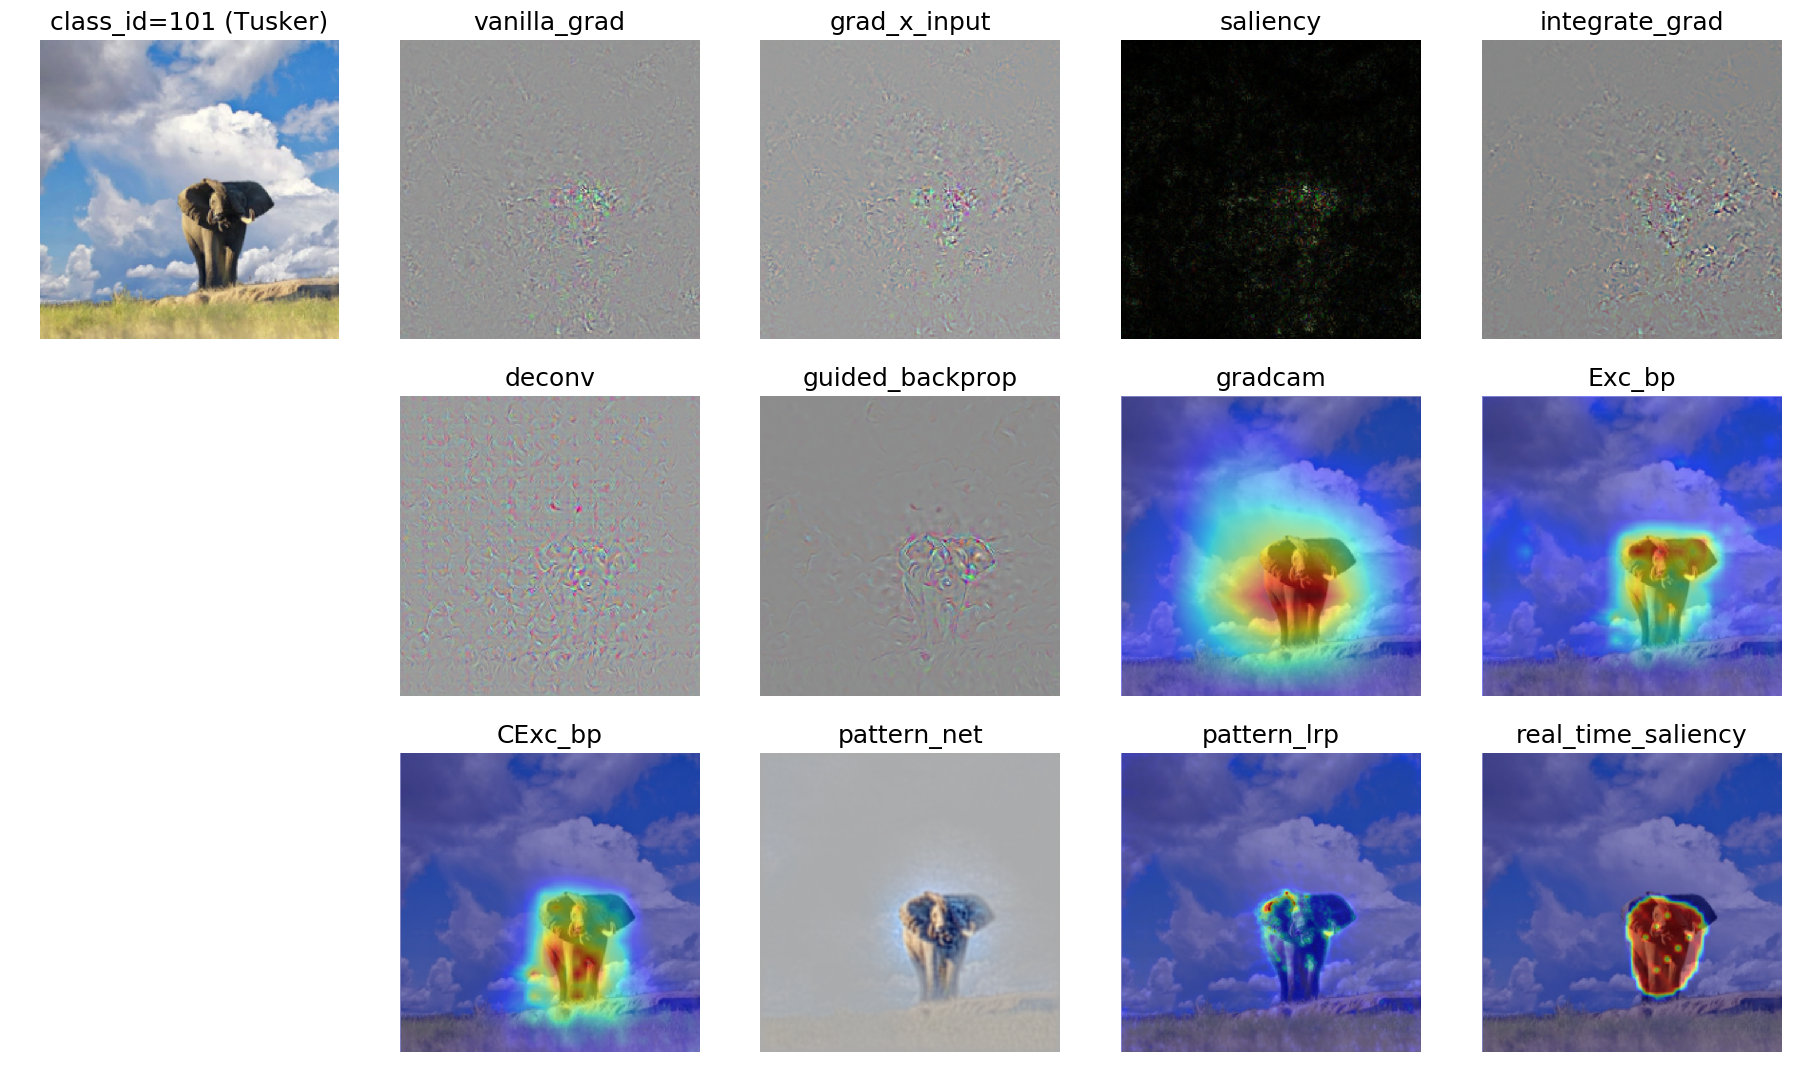
\includegraphics[width=14cm]{images/tusker_saliency.png}
\caption{Examples of some interpretability methods for image classification \cite{visualattribution}}
\label{classification_methods}
\end{figure}

These methods focus on providing explanations and interpretability of classification problems for datasets like ImageNet \cite{imagenet_cvpr09} or MNIST \cite{lecun1998gradient}. Classification means that an algorithm can tell what is displayed on an image, e.g. if and what kind of disease is visible on a x-ray or MRI scan.

\section{Image segmentation}
Image segmentation is different from classification in the way that the algoriths do not detect what is visible on a picture, but instead mark a region (the segment) in an image where it thinks something is visible. For example in self driving cars, it is important to know where another car or a pedestrian is in front of the car is. 

In the medical imaging field, one applications is the segmentation of tumors in MRI scans.

\section{Interpretability on image segmentation}
The interpretability of image segmentation task is nearly inexistent. In many cases this is understandable, because the interpretability methods would generate an image very similar to the actual segment. For example, in detecting pedestrians for self driving cars, the interpretability method would just mark the pedestrian. Only in cases where the network has not yet reached a good accuracy, other pixels in the image would be marked by the method.

In other fields like medical imaging, it is possible or even desirable that a neural network looks at other parts of an image to decide if a part should be segmented. An example for this is the search for tumors on MRI scans of the human brain. The human brain is physically symmetric. When a tumor is growing on one side of the brain, the brain is no longer symmetric. A physician and possibly also neural networks can use this property to detect and segment tumors.

\section{Goals}
The goal of this thesis is to take the existing methods for image classification and modify them so they can work on image segmentation tasks. This includes the following tasks:
\begin{itemize}
    \item Research existing methods for image classification
    \item Asses if the found methods can be modified for image segmentation
    \item Modify the methods for image segmentation
    \item Build and train a neural network on the BraTS brain tumor segmentation dataset
    \item Apply the modified methods on the trained neuronal network
    \item Analyze, evaluate and discuss the results
    \item Build a reusable Python library so other developers can easily use our modified messages
\end{itemize}

The second goal is providing the customer with images and visualization for use in their teaching material.

See appendix A for the full requirements specification.

\section{Customer}
The customer of this thesis is Mauricio Reyes and his team from the medical faculty of the University of Bern. Mr. Reyes is head Healthcare Imaging A.I. This thesis should help him and his team of master and PHD students to better understand the models they are developing.

\section{Source Code}
The source code of the thesis is available on GitHub:
\begin{itemize}
    \item Thesis source code (mostly jupyter notebooks): \url{https://github.com/andef4/thesis-code}
    \item Python library source code: \url{https://github.com/andef4/interpret-segmentation}
    \item Latex source for this document: \url{https://github.com/andef4/interpret-segmentation}
\end{itemize}

All source code is licensed under the permissive MIT license.


% \chapter{Interpretability methods}
% \label{chapter_methods}
Many different methods exist for the interpretation of neural networks. Most of them are specialized for deep convolutional neural networks that have images as an input and a range of classes as output.
% \section{Whitebox and blackbox methods}
Generally there are two types of methods for interpretability: Blackbox and whitebox. Blackbox methods like LIME or RISE do not need insight into the underlying model and can therefore be used on arbitrary network architectures and even non-deep learning technologies like decision trees.

Whitebox methods need to have access to the underling model (e.g. weights and activation values in a neural network), because they analyze a certain part of the network.

% \section{Methods overview}

\begin{tabular}{| p{7cm} | p{2.5cm} | p{6cm} | }
\hline
\textbf{Method} & \textbf{Blackbox method} & \textbf{PyTorch implementation available} \\ \hline

RISE\cite{Petsiuk2018rise} & Yes & Offical implementation is PyTorch \\ \hline
LIME\cite{ribeiro2016should} & Yes & No but feasible \\ \hline
Layer-wise Relevance Propagation (LRP) & No & Yes, but missing batch normalization\cite{lrppytorch} \\ \hline
DeepLIFT\cite{shrikumar2017learning} & No & Initial implementation in SHAP\cite{NIPS2017_7062} \\ \hline
Grad-CAM (Selvaraju 2017) & No & Many implementations \\ \hline
Meaningful Perturbation (Fong 2017)\cite{fong2017interpretable} & Yes & Implementation exitst \cite{fong2017implementation} \\ \hline

Prediction Difference Analysis \cite{todo} & ? & ? \\ \hline
PatternNet & ? & ? \\ \hline
SHAP DeepExplainer\cite{NIPS2017_7062} & No & No \\ \hline
SHAP KernelExplainer\cite{NIPS2017_7062} & Yes & Yes \\ \hline

Guided Backpropagation  & No & ? \\ \hline
Excitation Backprop (Zhang 2016)\cite{todo} & No & ? \\ \hline


\end{tabular}

% many implementations: https://github.com/yulongwang12/visual-attribution
% https://github.com/marcoancona/DeepExplain/blob/master/docs/comparison.png


% Poulin'06 Additive
% Baehrens'10 Gradient
% Symonian'13 Gradient
% Landecker'13 Contrib Prop
% Zeiler'14 Deconv
% Zeiler'14 Occlusions
% Caruana'15 Fitted Additive
% Haufe'15 Pattern
% Zhou'16 GAP
% Sundarajan'17 Int Grad

% \section{Method selection}
The initial selection of methods contain RISE, LIME and Grad-CAM.

LIME: Widly cited.
RISE: Proposed enhancement of LIME
Grad-CAM: Widly cited, many implementations as indicator of popularity and quality.

There are many methods, quite a few of them with PyTorch implementation.
=> visual attribution with generic code for multiple methods
If the modification of these methods for image segmentation is successful, additional methods will be selected.

% \section{LIME}

LIME \cite{ribeiro2016should} (Local Interpretable Model-Agnostic Explanations) is a black box interpretability method. Like all black box methods, LIME randomly changes features in the input data to detect which feature is relevant for a specific classification.

In the case of image classification, LIME does not modify single pixels, because this would generate too many different versions of the input.
Instead, LIME generates superpixels.

\begin{figure}[H]
    \centering
    \begin{subfigure}[t]{.35\textwidth}
        \centering
        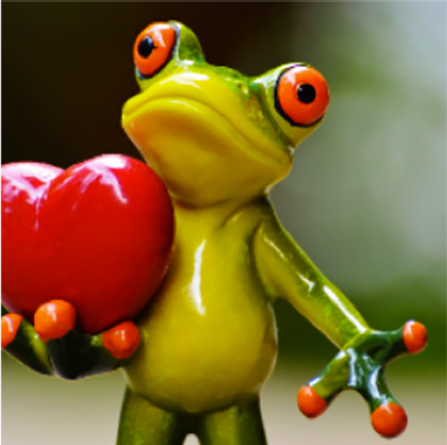
\includegraphics[width=\linewidth]{chapters/02_methods/images/frog1.png}
        \caption{Original image}
    \end{subfigure}\hspace{1.5cm}%
    \begin{subfigure}[t]{.35\textwidth}
        \centering
        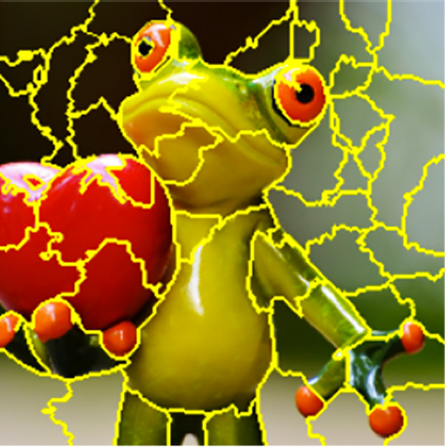
\includegraphics[width=\linewidth]{chapters/02_methods/images/frog2.png}
        \caption{Original image overlaid with superpixel boundaries}
    \end{subfigure}
    \caption{Superpixels generated for an input image. Superpixels are the features LIME analyzes to detect if they are relevant for the classification \cite{limeoreilly}.}
    \label{lime_superpixel}
\end{figure}


Superpixels are continuous regions on an image with a similar color. In the Python reference implementation, LIME uses the Quick Shift \cite{vedaldi2008quick} clustering algorithm to generate these superpixels. Figure \ref{lime_superpixel} shows superpixels overlaid on an example image.

\begin{figure}[H]
\centering
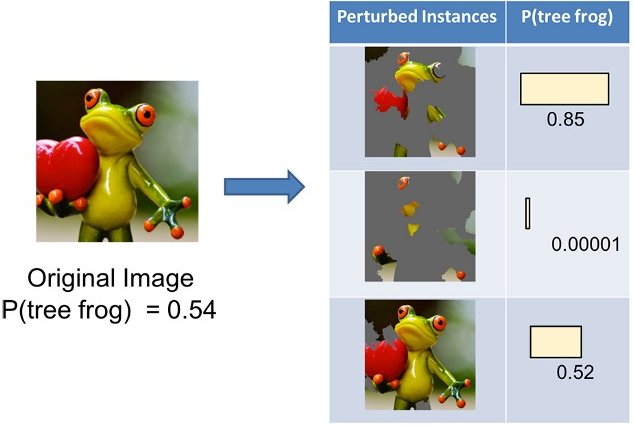
\includegraphics[width=8cm]{chapters/02_methods/images/lime1.jpg}
\caption{Left: Original image with detected class and probability. Right: Perturbed images generated by randomly turning off superpixels and their probability for the specific class.}
\label{lime_perturbed}
\end{figure}

In the next step, LIME generates input images by turning off multiple randomly selected superpixels. Turning off in this case means setting the color inside the superpixel to gray. The right image of Figure \ref{lime_perturbed} shows some examples of deactivated superpixels. The generated input images are then passed through the neural network and the changed probabilities of the relevant class(es) are recorded.

\begin{figure}[H]
\centering
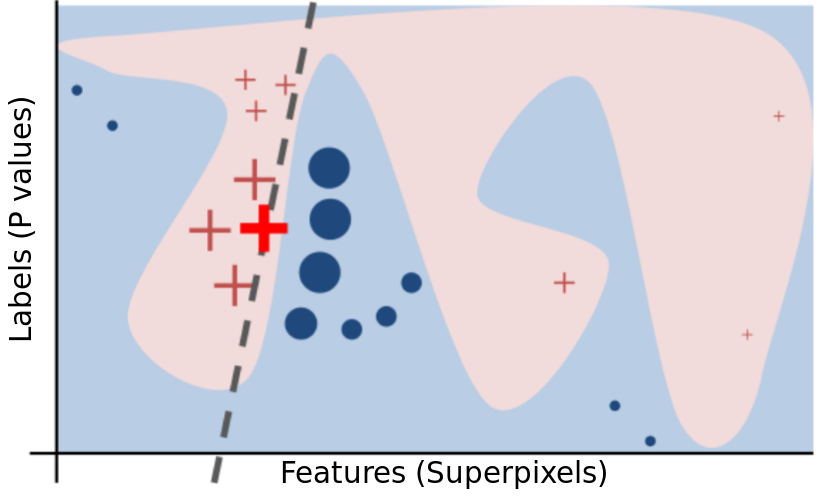
\includegraphics[width=8cm]{chapters/02_methods/images/lime2.png}
\caption{
The light red and blue background of the image represent the non-linear function of the underlying model.
The bright red cross represents the image that is explained. The smaller red crosses and blue circles represent
perturbed instances of image. The size of these symbols show the distance to the unchanged image. The x-axis represents the features, in the case of images these are the superpixels. The y-axis represents the output label of the neural network. The dashed line shows the fitted linear model.}
\label{lime_linear_regression}
\end{figure}

As a last step, LIME trains a linear regression model (Figure \ref{lime_linear_regression}) on this data: Superpixels represented as a binary vector on the x-axis and the corresponding neural network output for the specific class on the y-axis. The samples are weighted by distance to the original sample, because a linear model is trained which is accurate in the local environment of the unchanged image, but not further away because the underlying model is not linear. The coefficients of the linear model represent how important every superpixel is for the correct classification of the model.

For visualization, the coefficients are sorted by their value. Based on the superpixel count parameter given to LIME, the most important superpixels are drawn, all other superpixels are grayed out. 

Figure \ref{lime_dog} shows a visualization for three classes on a complex input image. Alternatively, the superpixel cluster is drawn over the input image with transparency.

\begin{figure}[H]
    \centering
    \begin{subfigure}[t]{.23\textwidth}
        \centering
        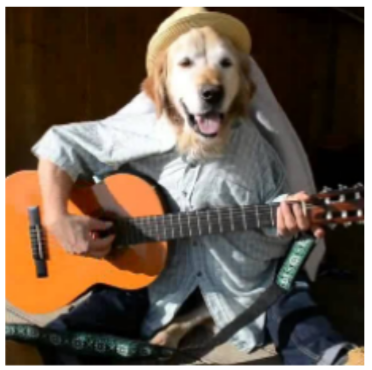
\includegraphics[width=\linewidth]{chapters/02_methods/images/lime_dog_1.png}
        \caption{Original image}
    \end{subfigure}\hfill%
    \begin{subfigure}[t]{.23\textwidth}
        \centering
        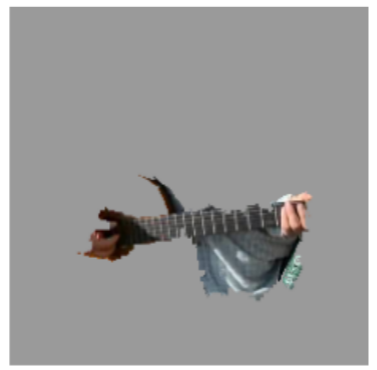
\includegraphics[width=\linewidth]{chapters/02_methods/images/lime_dog_2.png}
        \caption{Explain class "Electric guitar" (p=0.32)}
    \end{subfigure}\hfill%
    \begin{subfigure}[t]{.23\textwidth}
        \centering
        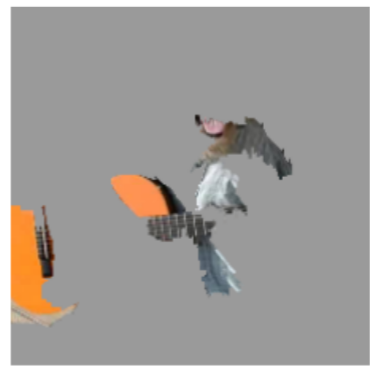
\includegraphics[width=\linewidth]{chapters/02_methods/images/lime_dog_3.png}
        \caption{Explain class "Acoustic guitar" (p=0.24)}
    \end{subfigure}\hfill%
    \begin{subfigure}[t]{.23\textwidth}
        \centering
        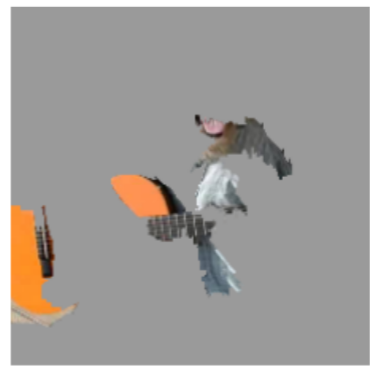
\includegraphics[width=\linewidth]{chapters/02_methods/images/lime_dog_3.png}
        \caption{Explain class "Labrador" (p=0.21)}
    \end{subfigure}
    \caption{Explaining the top 3 classes on an example image with LIME. The used neural network architecture is Inception trained on ImageNet \cite{ribeiro2016should}.}
    \label{lime_dog}
\end{figure}

% \section{RISE}

Like LIME, RISE\cite{Petsiuk2018rise} is a black box method and works by manipulating of the input images.

Instead of superpixels, RISE generates masks that are applied to the input images by multiplying the mask with the input image pixel values. Figure \ref{rise_mask0} and Figure \ref{rise_mask1} show two RISE masks applied to the same input image.

\begin{figure}[H]
    \centering
    \begin{subfigure}[t]{.32\textwidth}
        \centering
        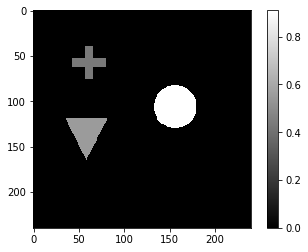
\includegraphics[width=\linewidth]{chapters/02_methods/images/rise/rise_original.png}
        \caption{Original image}
    \end{subfigure}\hfill%
    \begin{subfigure}[t]{.32\textwidth}
        \centering
        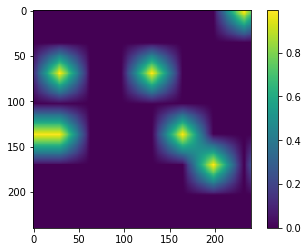
\includegraphics[width=\linewidth]{chapters/02_methods/images/rise/rise0_mask.png}
        \caption{RISE mask}
    \end{subfigure}\hfill%
    \begin{subfigure}[t]{.32\textwidth}
        \centering
        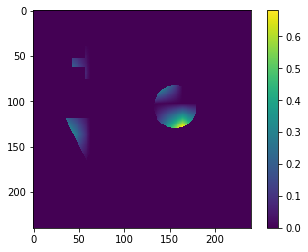
\includegraphics[width=\linewidth]{chapters/02_methods/images/rise/rise0_applied.png}
        \caption{RISE mask applied to original image by multiplication}
    \end{subfigure}
    \caption{By multiplication the input image (left) with a RISE mask (center), a modified input is generated (right).}
    \label{rise_mask0}
\end{figure}


\begin{figure}[H]
    \centering
    \begin{subfigure}[t]{.32\textwidth}
        \centering
        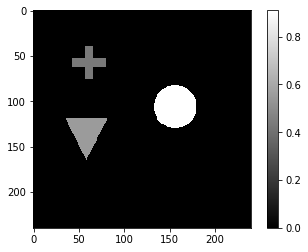
\includegraphics[width=\linewidth]{chapters/02_methods/images/rise/rise_original.png}
        \caption{Original image}
    \end{subfigure}\hfill%
    \begin{subfigure}[t]{.32\textwidth}
        \centering
        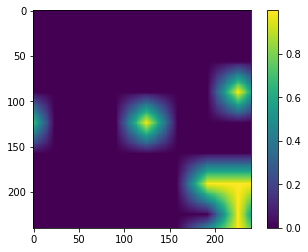
\includegraphics[width=\linewidth]{chapters/02_methods/images/rise/rise1_mask.png}
        \caption{RISE mask}
    \end{subfigure}\hfill%
    \begin{subfigure}[t]{.32\textwidth}
        \centering
        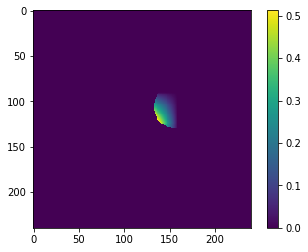
\includegraphics[width=\linewidth]{chapters/02_methods/images/rise/rise1_applied.png}
        \caption{RISE mask applied to original image by multiplication}
    \end{subfigure}
    \caption{By multiplication the input image (left) with a RISE mask (center), a modified input is generated (right). In comparison fo Figure \ref{rise_mask0}, this input image retains much less information.}
    \label{rise_mask1}
\end{figure}

The number of generated masks depend on the image resolution, e.g. for an image of size 240x240 pixels, 3000 masks generate good results. All masks are applied to the input image to generate new input images. The modified images are passed through the neural network and their classification scores for a specific class are recorded. A high classification score for a class on a modified input image means that the pixels preserved by the mask are important for the classification.

To visualize the results, the classification scores and masks are summed up and converted into a heat map. Figure \ref{rise_explanation} shows how the summing up works: The masks are multiplied with the classification score returned by running the masked image through the neural network. In Figure \ref{rise_explanation} for example, the leftmost mask was applied to an image, the image was run through the network and the network returned the value 0.7 for the first class. The next step is summing up all the values from the same cell into one matrix (image (c) in Figure \ref{rise_explanation}). In the actual implementation, the multiplication of the masks with the output values and summing up into one matrix is done with one matrix multiplication step.

\begin{figure}[H]
    \centering
    \begin{subfigure}[t]{\textwidth}
        \centering
        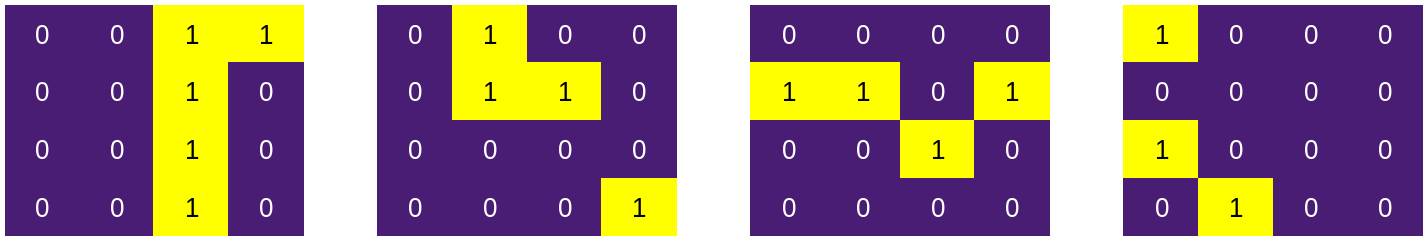
\includegraphics[width=\linewidth]{chapters/02_methods/images/rise/explain_rise_masks.png}
        \caption{Sample RISE masks}
    \end{subfigure}
    \begin{subfigure}[t]{\textwidth}
        \centering
        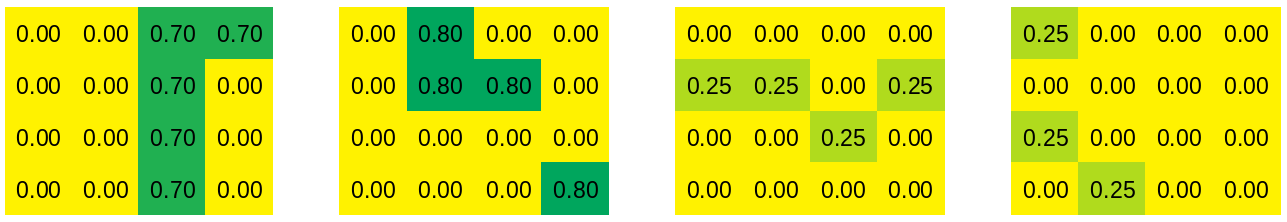
\includegraphics[width=\linewidth]{chapters/02_methods/images/rise/explain_rise_result.png}
        \caption{Masks multiplied by the classification value returned by the neural network after running the masked images through it}
    \end{subfigure}\hfill
    \begin{subfigure}[t]{.5\textwidth}
        \centering
        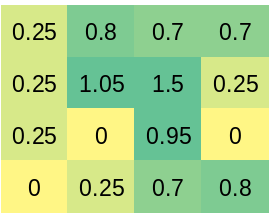
\includegraphics[width=\linewidth]{chapters/02_methods/images/rise/explain_rise_saliency.png}
        \caption{Saliency map generated by summing up all values for the same cell of the results in (b). E.g. second row second column is 0 + 0.8  + 0.25 + 0 = 1.05.}
    \end{subfigure}
    \caption{RISE masks (a) are multiplied by classification value returned by the network for the masked images (b). The same cell in theses matrices are summed up to generate a new matrix (c).}
    \label{rise_explanation}
\end{figure}

To visualize the generated matrix, the data is upscaled to the original image size and displayed as a heatmap by mapping the values to a color map. Figure \ref{rise_example} shows some examples for visualization of the RISE output for specific classes.

\begin{figure}[H]
\centering
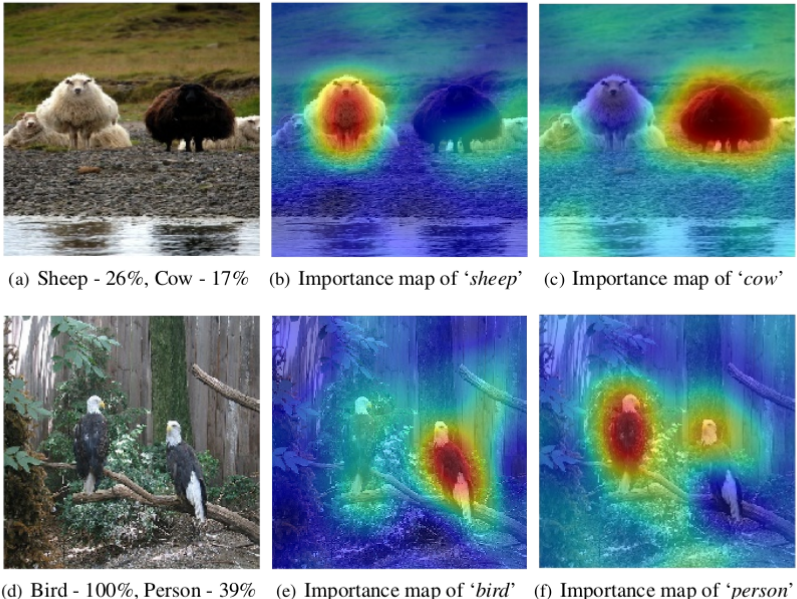
\includegraphics[width=12cm]{chapters/02_methods/images/rise/sheep.png}
\caption{Image from original paper explaining some classes}
\label{rise_example}
\end{figure}

% \section{Grad-CAM}
Grad-CAM\cite{selvaraju2017grad} (Gradient-weighted Class Activation Mapping) is a white box method, it requires insight into the convolutional neural network architecture and is therefore only applicable on CNNs. The method generates a heat map similar to RISE. Figure \ref{grad_cam_cat} and Figure \ref{grad_cam_dog} are outputs of Grad-CAM on an example image.

\begin{figure}[H]
    \centering
    \begin{subfigure}{.5\textwidth}
        \centering
        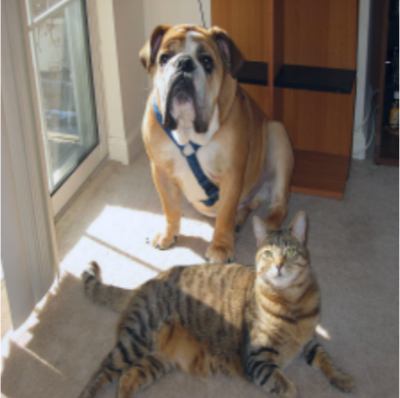
\includegraphics[width=0.7\linewidth]{chapters/02_methods/images/grad-cam-original.png}
        \caption{Original image}
    \end{subfigure}\hfill%
    \begin{subfigure}{.5\textwidth}
        \centering
        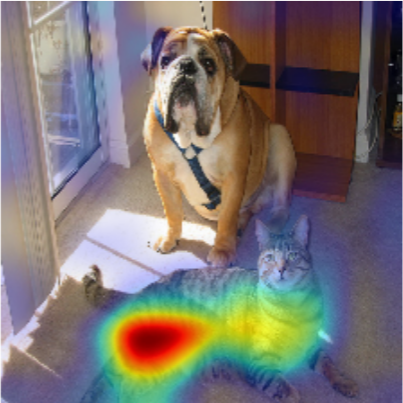
\includegraphics[width=0.7\linewidth]{chapters/02_methods/images/grad-cam-cat.png}
        \caption{Grad-CAM explanation for class cat}
    \end{subfigure}
    \caption{Grad-CAM applied on an image with multiple valid classes. Explanation for class cat.}
    \label{grad_cam_cat}
\end{figure}

\begin{figure}[H]
    \centering
    \begin{subfigure}{.5\textwidth}
        \centering
        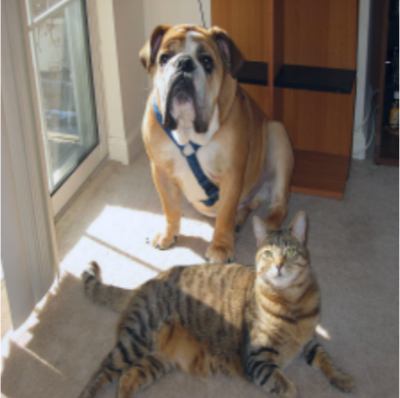
\includegraphics[width=0.7\linewidth]{chapters/02_methods/images/grad-cam-original.png}
        \caption{Original image}
    \end{subfigure}\hfill%
    \begin{subfigure}{.5\textwidth}
        \centering
        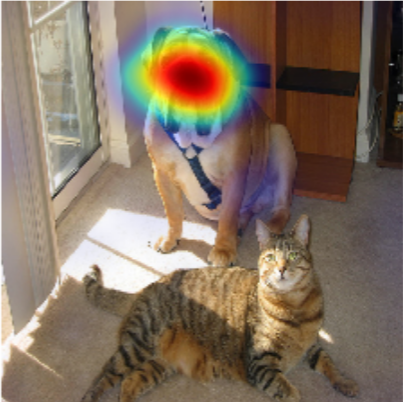
\includegraphics[width=0.7\linewidth]{chapters/02_methods/images/grad-cam-dog.png}
        \caption{Grad-CAM explanation for class dog}
    \end{subfigure}
    \caption{Grad-CAM applied on an image with multiple valid classes. Explanation for class dog.}
    \label{grad_cam_dog}
\end{figure}

The main parameter for this method is which convolutional layer of the neural network that should be analyzed. Figure \ref{grad_cam_explanation} shows a schematic of the inner working of Grad-CAM for a layer: The feature map (i.e. the result of applying the convolution kernels on the channel input) of the specified convolutional layer is extracted. Every channel of the feature map is weighted, based on how much it influences the final output value of the network for a specific class. Finally, the weighted channels are summed up, run trough ReLU and converted to a heat map by upsamling. The ReLU is applied to remove pixels which negativly impact the class output.

\begin{figure}[H]
\centering
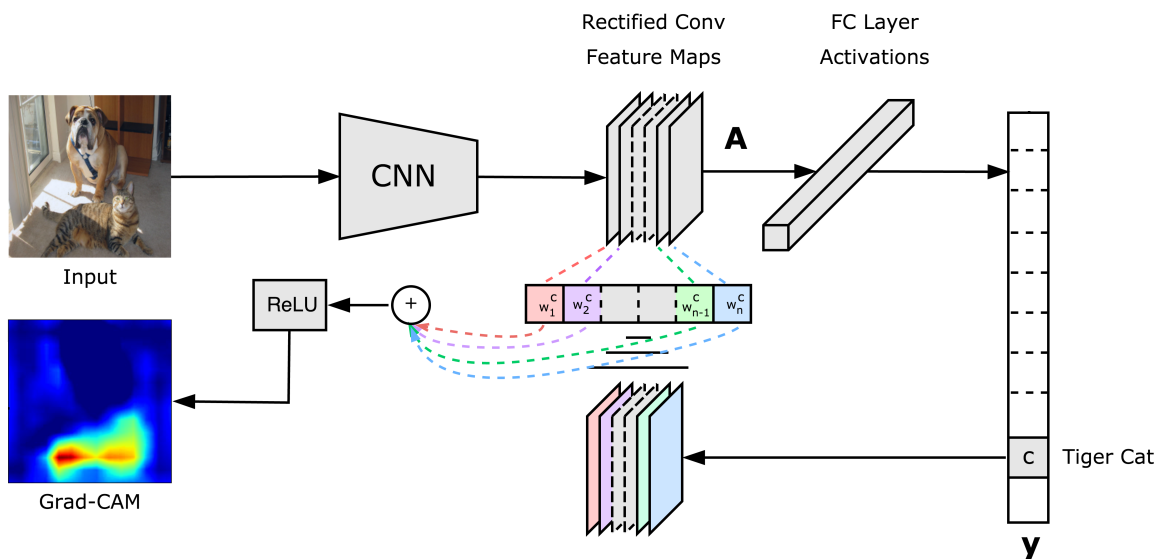
\includegraphics[width=12cm]{chapters/02_methods/images/grad-cam.png}
\caption{Grad-CAM in action: The feature map of a specific network layer is extracted, each channel weighted by the activation of the expected class, summed up and converted into a heat map}
\label{grad_cam_explanation}
\end{figure}



% \chapter{Classification}
% Almost all interpretability methods work on image classification tasks. To learn how these methods are applied, how they work and what output they generate, the first step in this work is applying these methods on a classification task. We chose a dataset from the medical imaging field: The NIH (National Institutes of Health, United States) chest X-ray dataset \cite{wang2017chestx}.

We downloaded the dataset, trained a neural network on the dataset and applied the selected methods described above.

\section{NIH Chest X-ray dataset}
The NIH Chest X-ray dataset contains 112,120 X-ray scans from 30,805 unique patients \cite{nihchestxraykaggle}. Every scan has one or more disease labels. Figure \ref{chest_xray_sample} show three sample images from the dataset.

\begin{figure}[h]
\centering
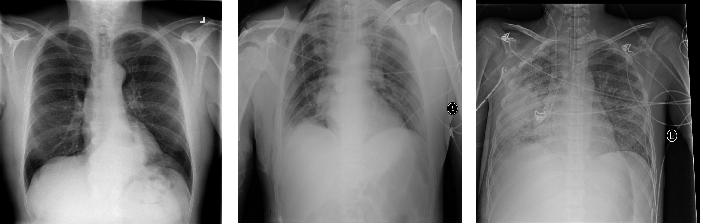
\includegraphics[width=14cm]{chapters/03_classification/images/chest-x-ray.png}
\caption{Examples for the NIH Chest X-ray dataset}
\label{chest_xray_sample}
\end{figure}

\section{Model Training}
We decided to train a model based on an existing neural network architecture, because building a state of the art architecture is very hard and not the focus of this thesis.

The detailed results of the training sessions are available in the results directory of the GitHub repository: \href{https://github.com/andef4/thesis-code/tree/master/nhs-chest-xray/results/}{nhs-chest-xray/results}.

\subsection{Inception ResNet v2}
\nblink{nhs-chest-xray/inception\_resnetv2.ipynb}

We chose Inception ResNet v2 \cite{szegedy2017inception} as the architecture. This is modern neural network built for image analysis and generally trained on the ImageNet dataset.
The ResNet variant of the Inception architecture delivers similar performance as the normal Inception model, but with significantly reduced training time.

\nblink{nhs-chest-xray/preprocess.ipynb}
The preprocessing steps required to use this architecture are resizing the images to 299x299 pixels and converting the gray-scale images to color images.
We also tried to modify the network to directly use gray-scale images, but this was not successful because the network architecture is built for three channel images.

We initially trained the network on a smaller subset (5607 image) of the dataset. The maximum reached validation accuracy was 40\%. The training times for the small training subset
were already very long, we therefore decided to abandon the Inception architecture for now and use a ResNet based architecture instead.

\subsection{ResNet}
\nblink{nhs-chest-xray/resnet.ipynb}

The first test of ResNet50 \cite{he2016deep} with pretrained parameters (trained on ImageNet) on the sample dataset showed fast training times but low accuracy. Training the network from scratch showed promising validation accuracy, which started to decrease on later epochs. The training accuracy was still increasing, this is therefore a clear indicator that the neural network is overfitting. We decided to change the architecture to ResNet18 which is a smaller ResNet variant with fewer parameters and should be less susceptible to overfitting.

The first training run of ResNet18 with the sample dataset looked promising, so we moved to train the network on the full dataset. The results were underwhelming, with the validation accuracy maxing out at 23\%.

\subsection{Single label only}
The NIH Chest X-ray dataset is a multi class dataset. This means a single image can contain labels for multiple disease. Training models for such datasets is much harder than training datasets where each image only has one label. We therefore decided to remove all images which contain multiple labels and only train on images with one label.

We did multiple iterations on the full dataset with ResNet18, experimenting with different parameters:
\begin{itemize}
    \item Running on sample dataset vs. full dataset
    \item Using SGD optimizer instead of Adam
    \item Using pretrained model vs. from scratch model
    \item Use data augmentation on the input (color jitter, random horizontal flip)
\end{itemize}

None of these parameters changed the validation accuracy significantly, always peaking around 60\% to 65\% training accuracy for the sample dataset.

\subsection{Densenet}
\nblink{nhs-chest-xray/densenet.ipynb}

Researching what other people did to train a model for this dataset, we came across the CheXNet \cite{rajpurkar2017chexnet} paper and an implementation of the paper in PyTorch \cite{chexnetpytorch}.

The paper uses the Densenet \cite{huang2017densely} architecture. An implementation of Densenet is available in PyTorch. The implementation of the paper provided a pretrained model, but loading the saved model did not work, because the used version of PyTorch was old and incompatible with ours.

\subsection{Retrain densenet}
\nblink{nhs-chest-xray/densenet\_singleclass.ipynb}

After fixing multiple implementation errors (not correctly setting the output class count, assigning of classes to output neurons not the same in test vs. validation set), we started to get acceptable accuracy rates for the Densenet implementation, peaking around 55\% accuracy.

\subsection{Only images with actual diagnosis}
The implementation of the CheXNet paper displayed an accuracy table per class. We decided to do the same for our implementation. We quickly discovered that only the "No findings" class was accurate, an all other classes had zero correct classifications. The "No findings" class is by far the biggest class in the dataset. For the neural network to get a good result, the easiest way is to just declare all images to be in the class "No findings".

We removed the "No findings" class from the dataset and retrained both the ResNet18 and the Densenet implementation, getting similar results of around 30\% accuracy.

\subsubsection{Weighted classes}
The dataset still has a class imbalance, even with the "No findings" class removed. To counter this problem, we calculated the 
% \section{Analyzing the network output}
\nblink{nhs-chest-xray/analyze/find\_best\_images.ipynb}
\nblink{nhs-chest-xray/analyze/find\_best\_images\_with\_bounding\_boxes.ipynb}
Because our trained network still has a low accuracy (around 33\%), we wanted to find correctly classified images with a high certainty.

Some images of the dataset also contain bounding boxes where a specific diagnosis is visible. This is useful to compare the output
of our interpretability methods with the bounding boxes created by physician.

\nblink{nhs-chest-xray/analyze/accuracy\_per\_class.ipynb}

We also calculated the accuracy for every class in the dataset, see Table \ref{chestxrayaccuracy}.

\begin{table}[H]
\begin{center}
\begin{tabular}{ | l | l | }
\hline
Atelectasis & 0.116105 \\ \hline
Cardiomegaly & 0.180380 \\ \hline
Consolidation & 0.022869 \\ \hline
Edema & 0.064935 \\ \hline
Effusion & 0.447301 \\ \hline
Emphysema & 0.062295 \\ \hline
Fibrosis & 0.028409 \\ \hline
Hernia & 0.133333 \\ \hline
Infiltration & 0.703153 \\ \hline
Mass & 0.203160 \\ \hline
Nodule & 0.102845 \\ \hline
Pleural Thickening & 0.058252 \\ \hline
Pneumonia & 0.000000 \\ \hline
Pneumothorax & 0.086044 \\
\hline
\end{tabular}
\caption{Table with accuracy for every class for the DenseNet model.}
\label{chestxrayaccuracy}
\end{center}
\end {table}

% \section{Applying RISE}
Problem: returned classes from RISE do not match with precalculated classes
=> normalize was not applied on find\_best\_images.
=> use same function on all image loaders

\nblink{nhs-chest-xray/analyze/rise.ipynb}
\nblink{nhs-chest-xray/analyze/rise\_bounding\_boxes.ipynb}

\subsection{Results}
\begin{figure}[H]
\centering
\caption{RISE example 1}
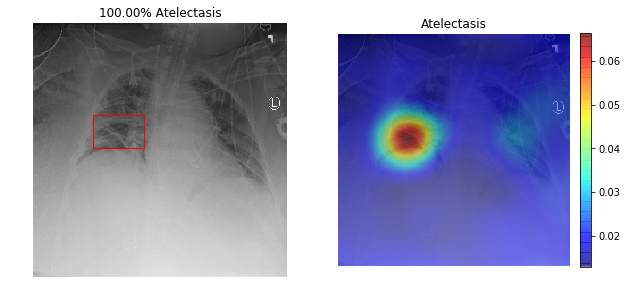
\includegraphics[width=12cm]{chapters/03_classification/images/rise_0.png}
\end{figure}

\begin{figure}[H]
\centering
\caption{RISE example 2}
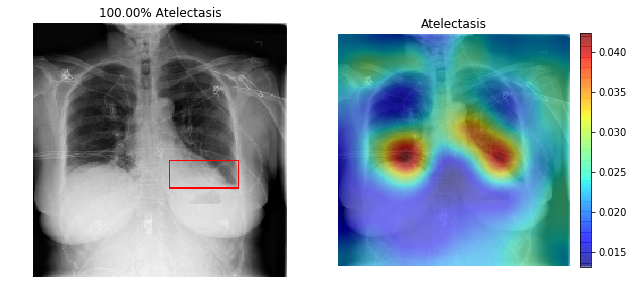
\includegraphics[width=12cm]{chapters/03_classification/images/rise_2.png}
\end{figure}

\begin{figure}[H]
\centering
\caption{RISE example 3}
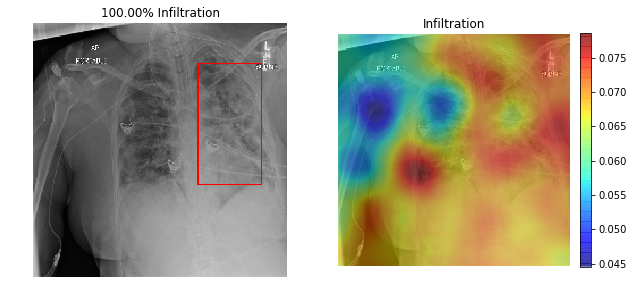
\includegraphics[width=12cm]{chapters/03_classification/images/rise_8.png}
\end{figure}

\subsection{Discussion}
Looks good for most, some (like the last image) are very bad.

\subsection{Conclusion}
Works good for most of the things, returns good quality, returns results for multiple classes at once which is probably helpful for segmentation
% \section{Applying LIME}
\nblink{nhs-chest-xray/analyze/lime.ipynb}

Implementing LIME on the NIH Chest X-ray dataset with the DenseNet model was straightforward. The refence implementation is published on PyPI (Python Packaging Index) and can be installed with the pip Python package manager. Examples how 



, because the reference implementation of RISE on GitHub \cite{risegithub} already
containes a working implementation for PyTorch. The implementation was not published on the Python Packaging Index, so the code had to be downloaded and added into our GitHub repository.


\subsection{Results}
\begin{figure}[H]
\centering
\caption{Scan 0 LIME output}
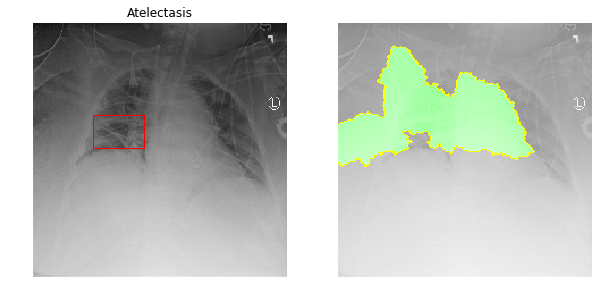
\includegraphics[width=12cm]{chapters/03_classification/images/lime_0.png}
\end{figure}

\begin{figure}[H]
\centering
\caption{Scan 2 LIME output}
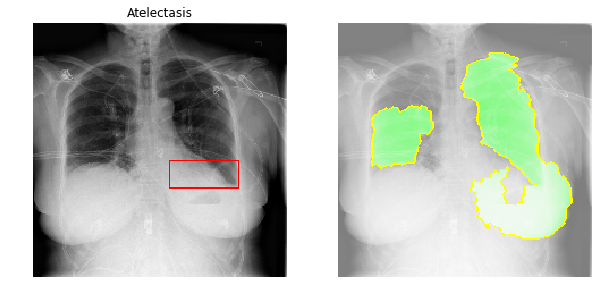
\includegraphics[width=12cm]{chapters/03_classification/images/lime_2.png}
\end{figure}

\begin{figure}[H]
\centering
\caption{Scan 8 LIME output}
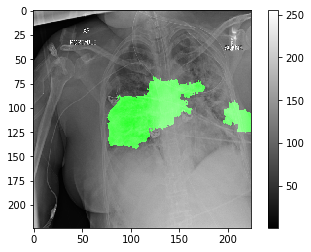
\includegraphics[width=12cm]{chapters/03_classification/images/lime_8.png}
\end{figure}

\subsection{LIME configuration}
\nblink{nhs-chest-xray/analyze/lime\_num\_features.ipynb}

\begin{figure}[H]
\centering
\caption{LIME Superpixel count: 1, 3, 6, 9}
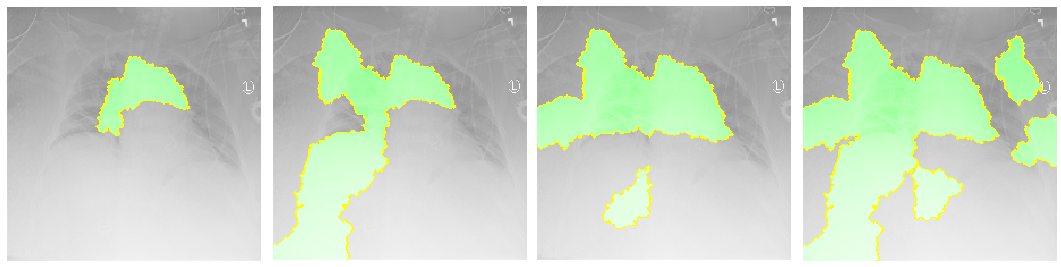
\includegraphics[width=14cm]{chapters/03_classification/images/lime-superpixel.png}
\end{figure}

\subsection{Discussion}

% \section{Applying Grad-CAM}
\nblink{nhs-chest-xray/analyze/grad-cam.ipynb}

An implementation of Grad-CAM is available in the Visual Attribution on GitHub \cite{visualattribution}. Visual Attribution is not available on PyPI We therefore copied the relevant code into our own GitHub repository. Visual Attribution is built on top of PyTorch, so the integration into our project was simple. Grad-CAM was run on the last layer before the linear (dense) output layer, which is a batch normalization layer. The output shape of a batch normalization layer that follows a convolutional layer is the same as the convolutional layer. Grad-CAM can therefore be applied on these too. We also tried running on the last real convolutional layer, with much worse results.

\begin{figure}[H]
    \centering
    \begin{subfigure}[t]{.45\textwidth}
        \centering
        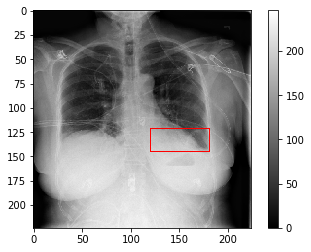
\includegraphics[width=\linewidth]{chapters/03_classification/images/rise1_bbox.png}
        \caption{Original image with bounding box added by a physician}
    \end{subfigure}\hspace{1cm}%
    \begin{subfigure}[t]{.45\textwidth}
        \centering
        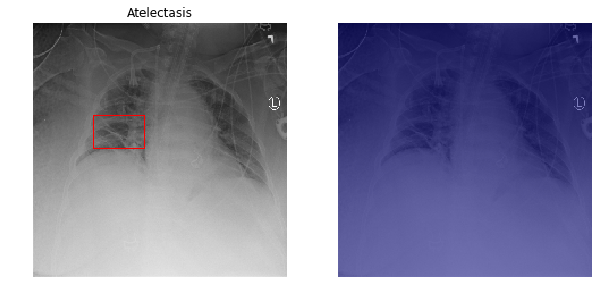
\includegraphics[width=\linewidth]{chapters/03_classification/images/grad-cam_0.png}
        \caption{LIME superpixels representing important regions for the classification}
    \end{subfigure}
    \caption{The left image shows the input image with the bounding box added by the physician. The right image shows the output of Grad-CAM, which in this case is blank.}
\label{grad_cam_example_1}
\end{figure}

\begin{figure}[H]
    \centering
    \begin{subfigure}[t]{.45\textwidth}
        \centering
        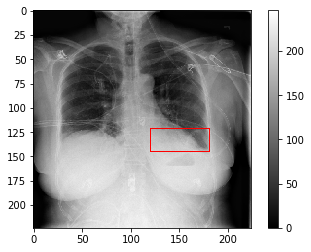
\includegraphics[width=\linewidth]{chapters/03_classification/images/rise1_bbox.png}
        \caption{Original image with bounding box added by a physician}
    \end{subfigure}\hspace{1cm}%
    \begin{subfigure}[t]{.45\textwidth}
        \centering
        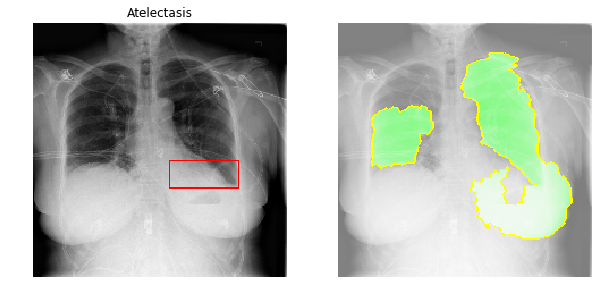
\includegraphics[width=\linewidth]{chapters/03_classification/images/lime_2.png}
        \caption{LIME superpixels representing important regions for the classification}
    \end{subfigure}
    \caption{The left image shows the input image with the bounding box added by the physician. The right image shows the output of Grad-CAM which contains the bounding box in the region detected as important, but the region is much bigger and its center outside of the bounding box.}
\label{grad_cam_example_2}
\end{figure}

\begin{figure}[H]
    \centering
    \begin{subfigure}[t]{.45\textwidth}
        \centering
        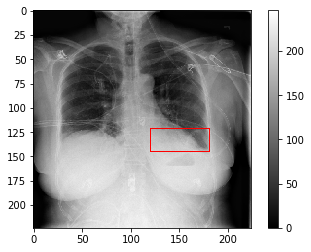
\includegraphics[width=\linewidth]{chapters/03_classification/images/rise1_bbox.png}
        \caption{Original image with bounding box added by a physician}
    \end{subfigure}\hspace{1cm}%
    \begin{subfigure}[t]{.45\textwidth}
        \centering
        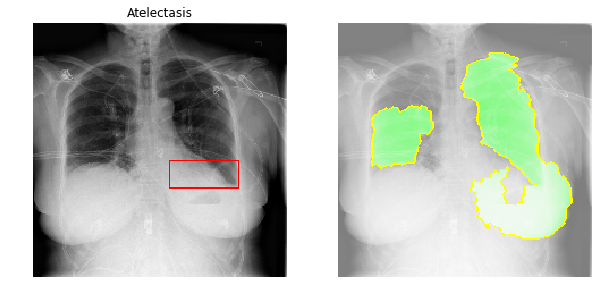
\includegraphics[width=\linewidth]{chapters/03_classification/images/lime_2.png}
        \caption{LIME superpixels representing important regions for the classification}
    \end{subfigure}
    \caption{The left image shows the input image with the bounding box added by the physician. The right image shows the output of Grad-CAM. The center of the output matches the bounding box.}
\label{grad_cam_example_3}
\end{figure}

\subsection{Discussion}
As seen in Figure \ref{grad_cam_example_1}, the output of Grad-CAM can be completely blank. This happens in 7 out of 21 tested images. The cause for this could not be found.

Other examples like Figure \ref{grad_cam_example_2} and Figure \ref{grad_cam_example_3} look acceptable, sometimes closely matching the bounding boxes.

\subsection{Conclusion}
The main problem with Grad-CAM is that it does not generate any output on 33\% of all images. If it actually generates output, Grad-CAM delivers usable output which most of the time marks a big part of the image as relevant for the correct classification.

% \section{Discussion}
Comparing all three algorithms, there is no clear picture which one performs the best.

From the black box methods, RISE looks to perform better, especially when looking at more example images in the linked Jupyter notebooks. It seems like
the superpixels generated by LIME do not work that well for this dataset, because the diseases do not show up as distinct uniform patches, but rather as faint color changes.

The adjustable superpixel count for the LIME output is problematic. Using only a small superpixel count works well when the network only looks at a small part of an image, but when it looks
at a big part, this will not show up until we use more superpixels. The size of the output should be decided by the method and not by the user of the method, because the user can only guess what
the correct superpixel count could be.

Grad-CAM has a strange problem where it does not generate a heat map for some images. A reason for this behaviour could not be found. If there is output,
the quality is quite high, but the marked regions are very big. In the Infiltration case (Figures \ref{lime_example_3}, \ref{rise_example_3}, \ref{grad_cam_example_3}, Grad-CAM delivers by far
the best output, especially compared to RISE.

A big advantage of Grad-CAM is its performance, which it has in common with all white box methods. The image only has to go trough the neural network once, recording activations and gradients in the process which are then analyzed in the end. In comparison, black box methods have to run many modified images trough the neural network, not just one.

\section{Conclusion}
Grad-CAM provided some good insights into the neural network and will be modified for image segmentation.

RISE performed better than LIME and does not use a configuration variable which is difficult to correctly set and will therefore be prioritized for the image segmentation modifications.


% \chapter{Segmentation}
% \section{Introduction}
To evaluate the modified methods, we need a dataset and a trained model where we can apply the methods.

The constituent Mauricio Reyes proposed the BraTS \cite{menze2015multimodal} dataset. This dataset contains
images of human brains taken with an MRI machine. The images are taken from patients which have brain tumors from the type
glioblastoma or lower grade glioma. The dataset contains four different types of images taken by the MRI machine (called modalities, the first images in Figure \ref{brats_example}).

\begin{figure}[H]
\centering
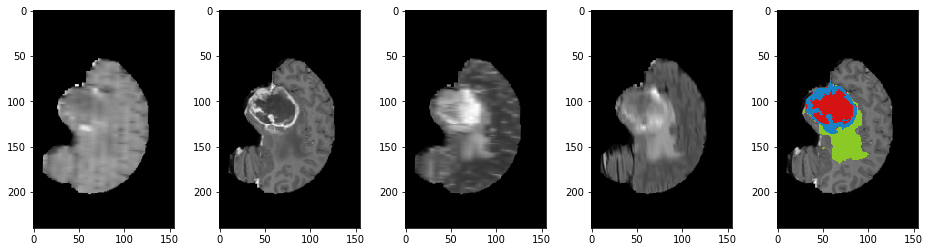
\includegraphics[width=14cm]{chapters/04_segmentation/images/brats.png}
\caption{One slice showing all 4 modalities and the tumor segmentation ground truth overlaid on the T1 contrast modality.}
\label{brats_example}
\end{figure}

In addition, the dataset contains ground truth labels. These labels mark the region in the brain where the tumor resides.
This segments are further divided into different tissue types each showing different states the tumor is in.
These labels were manually drawn by physicans and validated by experienced neuro-radiologists.

% \section{Medical background}
The brain scans in the BraTS\cite{menze2015multimodal} 2018 dataset were made with MRI scanners\cite{mriscanner}. 
An MRI scanner uses the fact that tissue consists mostly of water. Water molecules contain two hydrogen molecules,
each of which has one proton. A proton spins in a specific direction. When a strong magnet is applied to a proton, the proton starts to spin in the same direction as the magnet. 

An MRI scanner can generate a very precise and targeted magnetic field. When the magnet is deactivated, the protons go back into their resting position. Depending on the material a proton is part of (gray matter, necrotic tissue, cerebrospinal fluid  etc.), the resting position of the proton is different and a different amount of energy is released when the proton returns to its resting position. This radio frequency is measured by the MRI scanner and visualized as a scan. MRI scanners go through the brain in layers and generate a 2D image of every layer called a slice. The output of an MRI scanner is therefore a 3D volume.

\subsection{Slice modalities}
The BraTS dataset contains four different slice types, called modalities. These types are generated by specific settings of the MRI machine and by inserting a contrast enhancing fluid into the brain of the patient.

\subsubsection{T1}
For the T1 modality scan, the MRI machine measures the vertical movement of the protons when returning to their resting position. This modality mainly highlights fat and therefore contrast between fat and other tissue, e.g. nerve roots \cite{mriquora}. This modality only faintly shows tumor tissues, as seen in Figure \ref{medical_background_t1}.

\begin{figure}[H]
    \centering
    \begin{subfigure}{.5\textwidth}
        \centering
        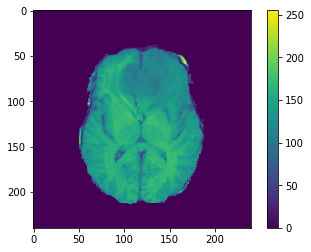
\includegraphics[width=\linewidth]{chapters/04_segmentation/images/medical_background/t1.png}
        \caption{T1 modality}
    \end{subfigure}%
    \begin{subfigure}{.5\textwidth}
        \centering
        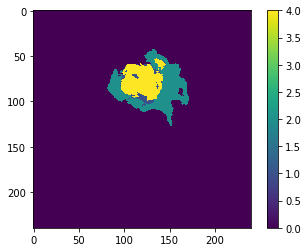
\includegraphics[width=\linewidth]{chapters/04_segmentation/images/medical_background/tumor.png}
        \caption{Tumor ground truth}
    \end{subfigure}
    \caption{The left image shows the T1 modality of a slice. There is only a small correlation with the gadolinium-enhancing (made visible with a contrast enhancement fluid) tumor tissue in the tumor ground truth (yellow, value 4) and also cerebrospinal fluid in the center lower half of the image.}
    \label{medical_background_t1}
\end{figure}



\subsubsection{T2}
The T2 modality measures the horizontal movement of the protons returning to their resting position. This modality highlights water, e.g. cerebrospinal fluid, but also edema tissue as seen in Figure \ref{medical_background_t2}.
\begin{figure}[H]
    \centering
    \begin{subfigure}{.5\textwidth}
        \centering
        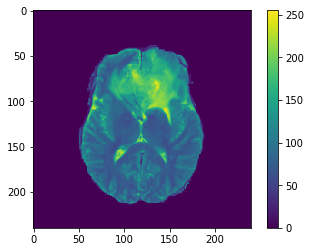
\includegraphics[width=\linewidth]{chapters/04_segmentation/images/medical_background/t2.png}
        \caption{T2 modality}
    \end{subfigure}%
    \begin{subfigure}{.5\textwidth}
        \centering
        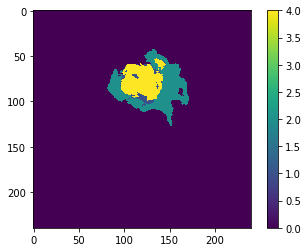
\includegraphics[width=\linewidth]{chapters/04_segmentation/images/medical_background/tumor.png}
        \caption{Tumor ground truth}
    \end{subfigure}
    \caption{The left image shows the T2 modality of a slice. Clearly visible is the edema of the tumor ground truth (turquoise, value 2.0).}
    \label{medical_background_t2}
\end{figure}



\subsubsection{T1 contrast enhanced}
Gadolinium is a chemical compound given to the patient during MRI scans that highlights areas of inflammation.
The scanner itself has the same setting as with a non-contrast enhanced T1 scan. The inflammed gadolinium enhanced tumor is clearly visible in Figure \ref{medical_background_t1ce}.

\begin{figure}[H]
    \centering
    \begin{subfigure}{.5\textwidth}
        \centering
        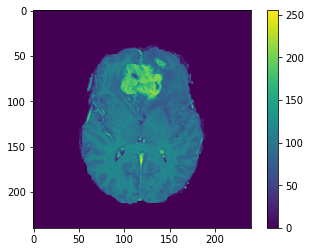
\includegraphics[width=\linewidth]{chapters/04_segmentation/images/medical_background/t1ce.png}
        \caption{T1 contrast enhanced}
    \end{subfigure}%
    \begin{subfigure}{.5\textwidth}
        \centering
        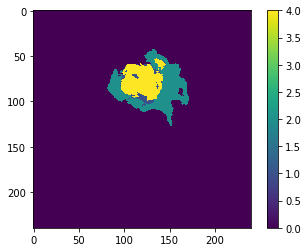
\includegraphics[width=\linewidth]{chapters/04_segmentation/images/medical_background/tumor.png}
        \caption{Tumor ground truth}
    \end{subfigure}
    \caption{The left image shows the T1 contrast enhanced modality of a slice. Clearly visible is the gadolinium enhanced tumor (yellow, value 4.0).}
    \label{medical_background_t1ce}
\end{figure}



\subsubsection{T2 FLAIR}
T2 FLAIR (Fluid-Attenuated Inversion Recovery) \cite{mribasics} is similar to the T2 modality. The difference to T2 is the much longer time between magnet pulses by the MRI machine.
The images are similar to the T2 images, but cerebrospinal fluid is much darker and actual tumor tissue is brighter, as seen in Figure \ref{medical_background_flair}. The disadvantage
of this method is the reduced sharpness of the image.

\begin{figure}[H]
    \centering
    \begin{subfigure}{.5\textwidth}
        \centering
        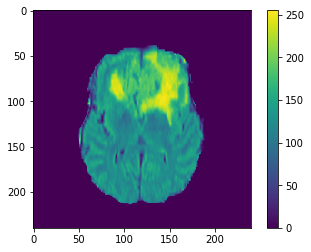
\includegraphics[width=\linewidth]{chapters/04_segmentation/images/medical_background/flair.png}
        \caption{FLAIR Modality}
    \end{subfigure}%
    \begin{subfigure}{.5\textwidth}
        \centering
        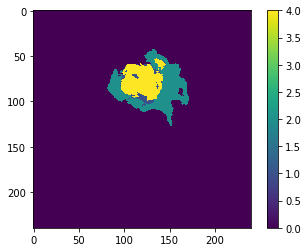
\includegraphics[width=\linewidth]{chapters/04_segmentation/images/medical_background/tumor.png}
        \caption{Tumor ground truth}
    \end{subfigure}
    \caption{The left image shows the FLAIR modality of a slice. Clearly visible is the edema of the tumor ground truth (turquoise, value 2.0), but also the other parts of the tumor.
    In comparison to T2, the cerebrospinal fluid in the lower half of the brain is almost black.}
    \label{medical_background_flair}
\end{figure}

% \section{BraTS 2018 dataset}
The BraTS dataset \cite{menze2015multimodal} contains MRI scans of the human brain. It is provided by the University of Pennsylvania (UPenn) but contains data from many different clinical institutes.
We use the 2018 version of the dataset, which contains new scans and revised ground truth segments.

\subsection{Data format}
The data is provided in the NIfTI file format (file ending *.nii.gz). It can be opened by the Python library NiBabel\cite{nibabel} which transforms the data into ordinary numpy arrays.

\subsection{Ground truth/labels}
The dataset contains ground truth segments with the following tissue types:

\begin{itemize}
    \item Gadolinium-enhancing tumor (ET - label value 4)
    \item Peritumoral edema (ED - label value 2),
    \item Necrotic and non-enhancing tumor core (NCR/NET - label value 1)
\end{itemize}

The labels are also saved in the NIfTI file format, using the integer values from above for every tissue type.

% \section{Preprocessing \& Slice selection}
\nblink{brats/02\_preprocess.ipynb}
\nblink{brats/03\_train\_test\_split.ipynb}


% \section{Neural network architecture}
\subsection{U-Net architecture}
The standard architecture for image segmentation tasks in the medical imaging field is the U-Net \cite{ronneberger2015u}.

Figure \ref{unet} shows the architecture of the U-Net. The left side is called the encoder, the right side the decoder.

The encoder part is a standard deep convolutional neural network, doing standard feature detection with continuously bigger features using convolutional layers.

The decoder part on the right side is used to actually generate the segmentation output. The max pooling in the encoder part made the processed image continuously smaller,
to detect bigger features. The decoder does the counterpart, it increases the image until is has (almost) the same size as the input image again. It not only uses
the smallest feature map produced by the last convolutional layer of the encoder, but also the feature maps of the last convolutional layer of every encoder block.
A block contains two convolutional layers and corresponding ReLU activation functions. The upscaling from one decoder block to the next (the green arrows in the diagram) are
implemented with standard image upscaling algorithms like bilinear upsampling.


https://github.com/milesial/Pytorch-UNet
https://github.com/usuyama/pytorch-unet

modifications: do not use deprectated functions

\begin{figure}[H]
\centering
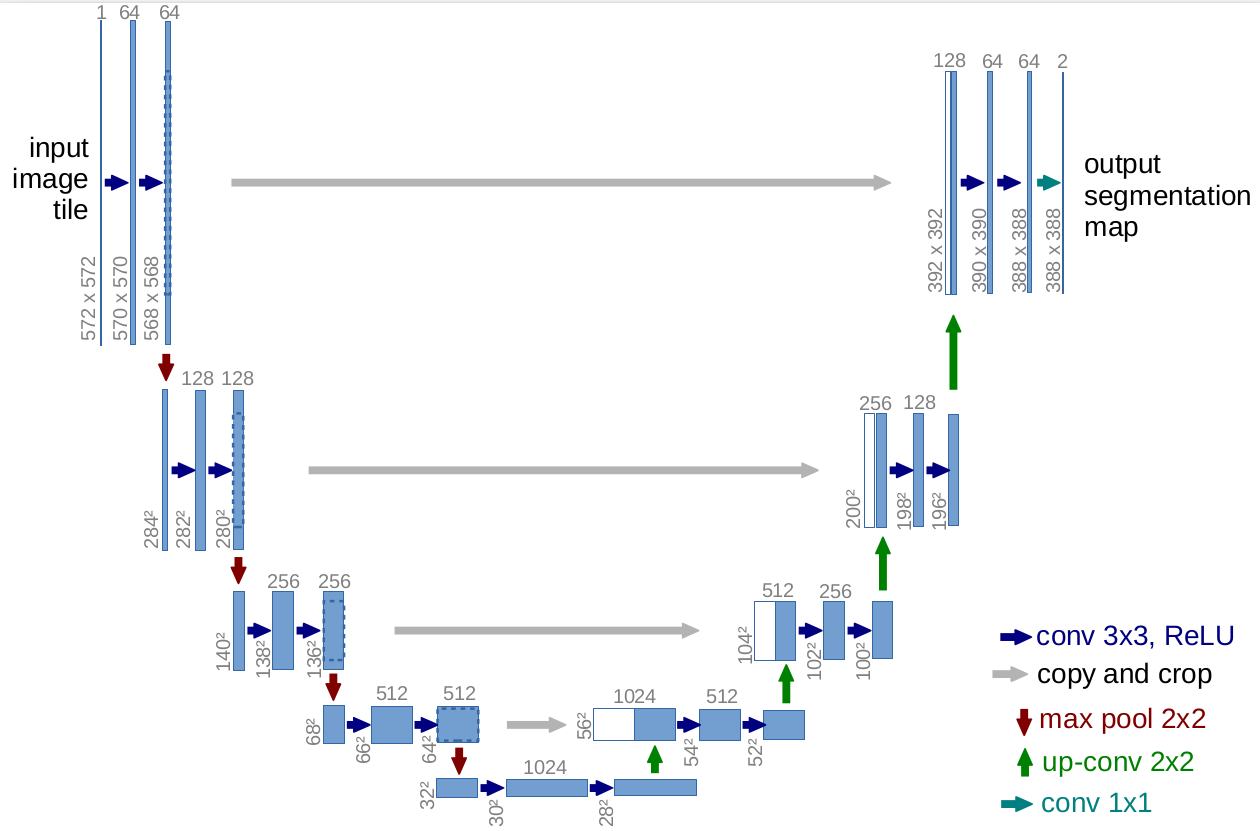
\includegraphics[width=14cm]{images/unet.png}
\caption{The U-Net architecture \cite{ronneberger2015u}.}
\label{unet}
\end{figure}

% \section{Training}
\nblink{brats/04\_basic\_unet.ipynb}
The detailed results of the training sessions are available in the results directory of the GitHub repository: \href{https://github.com/andef4/thesis-code/tree/master/brats/results/}{brats/results}.

The first try training the U-Net model showed good loss values soon after starting the training session. When we actually looked at the output of the network, the output was completely blank.

To avoid the lengthy process with evaluating different network architectures and parameters like in the classification model for the NIH Chest X-Ray dataset, we started to read different resources for enhancements of the basic U-Net architecture

The first change we implemented was correctly normalizing the input data by using a transform from the PyTorch library.
Retraining after this change showed similar low loss values as in the first attempt, with the same result when evaluating the network output - a blank image.

The second change we did after some investigation was the introduction of a batch normalization layer after every convolutional layer. The first training run after this change showed much worse loss numbers which decreased slowly.

We implemented the calculation of the Dice score (also called the F1 score) and the Hausdorff distance (see chapter \ref{hausdorff_distance_chapter} for an explanation) in addition to the loss value to have some more insight into the training process.

We let the training process run for around 4 hours. After that, the output images from the network looked very promising.

% \section{Evaluation}

\begin{figure}[H]
\centering
\caption{Comparing ground truth and network output}
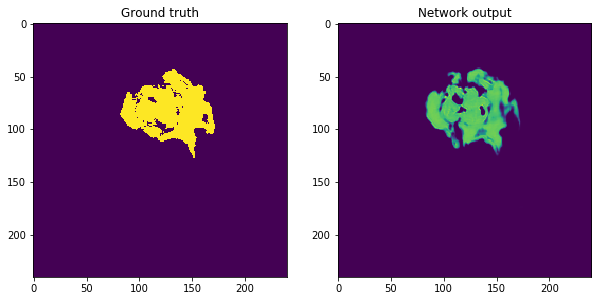
\includegraphics[width=12cm]{chapters/04_segmentation/images/network_output.png}
\end{figure}

\begin{figure}[H]
\centering
\caption{Confusion matrix visualization with binarized network output}
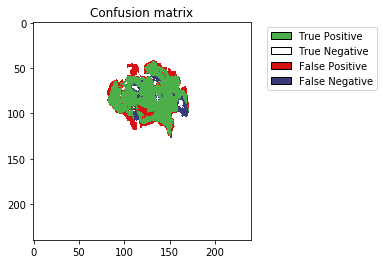
\includegraphics[width=10cm]{chapters/04_segmentation/images/confusion_matrix.png}
\end{figure}

% \clearpage

\section{Modifying and applying Grad-CAM}
\nblink{brats/07\_gradcam.ipynb}

The basic idea how to apply interpretability methods built for classification on image segmentation tasks is quite simple: The output of a classification model
is a list of confidence scores, one for every class the model can detect. In a segmentation task, the output is a list of pixels with an intensity value.
What we can do is interpret every output pixel as if was a separate class in a classification task.
In a classification task, we are only interested in the highest class value. In a segmentation task, we are interested why a specific pixel from the ground truth did
or did not show up in the network output.

As a first step, we can analyze a saliency map generated for a single class. In the following Result chapter, we analyze the pixel indicated by a red dot.

\clearpage

\subsection{Results}

Figure \ref{grad_cam_brats_result} shows the Grad-CAM output of multiple layers of the neural network. Grad-CAM for classification is applied on the last convolutional layer
of the network, but in this case this produced no output at all (Image (i) in the figure). We therefore decided to also analyze other layers (batch normalization and convolutional layers)
to see if there is any insight how the network came up with the output segmentation.

\begin{figure}[H]\ContinuedFloat
    \centering
    \begin{subfigure}{.32\textwidth}
        \centering
        \includegraphics[width=\linewidth]{chapters/04_segmentation/images/grad_cam_03.png}
        \caption{First batch norm layer of the first encoder block}
    \end{subfigure}\hfill%
    \begin{subfigure}{.32\textwidth}
        \centering
        \includegraphics[width=\linewidth]{chapters/04_segmentation/images/grad_cam_05.png}
        \caption{Second convolutional layer in the second encoder block}
    \end{subfigure}\hfill%
    \begin{subfigure}{.32\textwidth}
        \centering
        \includegraphics[width=\linewidth]{chapters/04_segmentation/images/grad_cam_14.png}
        \caption{First batch norm layer of the 4. encoder block}
    \end{subfigure}

    \begin{subfigure}{.33\textwidth}
        \centering
        \includegraphics[width=\linewidth]{chapters/04_segmentation/images/grad_cam_17.png}
        \caption{Second convolutional layer of the 5. encoder block}
    \end{subfigure}\hfill%
    \begin{subfigure}{.32\textwidth}
        \centering
        \includegraphics[width=\linewidth]{chapters/04_segmentation/images/grad_cam_24.png}
        \caption{First convolutional layer of the second decoder block}
    \end{subfigure}\hfill%
    \begin{subfigure}{.32\textwidth}
        \centering
        \includegraphics[width=\linewidth]{chapters/04_segmentation/images/grad_cam_29.png}
        \caption{Second convolutional layer of the third decoder block}
    \end{subfigure}

    \begin{subfigure}{.33\textwidth}
        \centering
        \includegraphics[width=\linewidth]{chapters/04_segmentation/images/grad_cam_30.png}
        \caption{First batch norm layer of the third decoder block}
    \end{subfigure}\hfill%
    \begin{subfigure}{.32\textwidth}
        \centering
        \includegraphics[width=\linewidth]{chapters/04_segmentation/images/grad_cam_34.png}
        \caption{First batch norm layer of the 4. decoder block}
    \end{subfigure}\hfill%
    \begin{subfigure}{.32\textwidth}
        \centering
        \includegraphics[width=\linewidth]{chapters/04_segmentation/images/grad_cam_36.png}
        \caption{Output convolutional layer}
    \end{subfigure}
    \caption{Grad-CAM output of the first pixel of the ground truth output segment (red pixel). No layers provided any significant insight into how the network came to the output segment.}
    \label{grad_cam_brats_result}
\end{figure}

\clearpage

\subsection{Discussion}
\nblink{brats/25\_flair\_threshold.ipynb}
None of the generated outputs provide good insight into the inner workings of the network. The output of the batch normalization layer of the third decoder (Image (g) in Figure \ref{grad_cam_brats_result}) shows the most promising output. But this output can easily be replicated by taking the FLAIR modality and applying a threshold, as seen in Figure \ref{grad_cam_treshold}.

\begin{figure}[H]
\centering
\includegraphics[width=8cm]{chapters/04_segmentation/images/flair_treshold.png}
\captionsetup{width=12cm}
\caption{FLAIR modality with an applied threshold of 170, setting all pixels lower than this value to zero. Shows a very similar shape as image (g) in Figure \ref{grad_cam_brats_result}}
\label{grad_cam_treshold}
\end{figure}


\subsection{Conclusion}
Because of these very underwhelming results, we decided to not modify Grad-CAM to work on multiple pixels and move to other methods.

% \section{Modifying and applying RISE (Single Pixel)}
\nblink{brats/06\_rise.ipynb}

The approach how to apply RISE on a segmentation task the same as with Grad-CAM in the last chapter. Pixels in the output of a segmentation model are equivalent to classes of a classification model.
As a first version, we only analyze a single pixel. We chose the first pixel in the tumor ground truth segment by iterating over the segment linearly until the first active pixel is found.


\subsection{Results}

\begin{figure}[H]
\centering
\includegraphics[width=8cm]{chapters/04_segmentation/images/rise_single_pixel.png}
\caption{Saliency map analyzing the topmost pixel in the scan, overlaid on the generated network output}
\label
\end{figure}



\subsection{Discussion}
looks correct, maybe a bit off => could be scaling

The produced output looks correct, the color blob is at the correct position. It clearly shows that the neural network looks at the correct location to generate the segmentation.
Apart from this basic correctness verification, no further insigt is provided by the saliency map, because the resolution generated by RISE is too low.

\subsection{Conclusion}
The generated output is low resolution but still helpful, we therefore decided to build a version of RISE which works on all pixels of the segmentation.

\section{Modifying and applying RISE (Multi Pixel)}
\nblink{17\_rise\_multipixel.ipynb}

TODO: implementation

\subsection{Results}
\begin{figure}[H]
    \centering
    \begin{subfigure}{.5\textwidth}
        \centering
        \includegraphics[width=\linewidth]{chapters/04_segmentation/images/rise_multipixel_max_1-0.png}
        \caption{ the text for a}
    \end{subfigure}%
    \begin{subfigure}{.5\textwidth}
        \centering
        \includegraphics[width=\linewidth]{chapters/04_segmentation/images/rise_multipixel_max_1-1.png}
        \caption{b}
    \end{subfigure}
    \caption{Explanation text}
\end{figure}

\subsection{Discussion}

\subsection{Conclusion}


% \chapter{Testnet}
% \section{Motivation}



\section{Introduction}
\nblink{brats/08\_testnet\_generate.ipynb}
\nblink{brats/09\_testnet\_train.ipynb}

\section{Applying RISE}
\nblink{brats/brats/10\_testnet\_rise.ipynb}
\nblink{brats/brats/11\_testnet\_rise\_segment\_ignore.ipynb}


\subsection{Results}
TODO Multipixel RISE results

\subsection{Discussion}
TODO: something is visible, but not good enough


\chapter{Hausdorf Distance masks}
\section{Introduction}
\nblink{brats/12\_rise\_masks.ipynb}

The results from applying RISE on our segmentations problems (BraTS and testnet) where underwhelming. While they showed a low resolution heat map output on both tasks,
on the testnet is missed out a big part (the right side of the image) which is very important for the correct generation of the segmentation output.

We suspect that this is caused by the low information entropy retained after applying a RISE mask on an image, as shown in Figure \ref{hdm_rise_mask}.
The basic idea of occluding a part of an image is not new and has been proposed by Zeiler et. al. in 2014 \cite{zeiler2014visualizing} in a highly cited paper.
Another similar method is Prediction Difference Analysis \cite{zintgraf2017visualizing} by Zintgraf et al.

Still, all investigated algorithms and methods were originally built for image classification tasks. We therefore propose a new method based on the same basic idea
of occluding parts of an image to see how it changes the output, but in a way that is specialized for image segmentation tasks. We named the method "Hausdorff distance masks".

\begin{figure}[H]
    \centering
    \begin{subfigure}[t]{.32\textwidth}
        \centering
        \includegraphics[width=\linewidth]{chapters/02_methods/images/rise/rise_original.png}
        \caption{Original image}
    \end{subfigure}\hfill%
    \begin{subfigure}[t]{.32\textwidth}
        \centering
        \includegraphics[width=\linewidth]{chapters/02_methods/images/rise/rise1_mask.png}
        \caption{RISE mask}
    \end{subfigure}\hfill%
    \begin{subfigure}[t]{.32\textwidth}
        \centering
        \includegraphics[width=\linewidth]{chapters/02_methods/images/rise/rise1_applied.png}
        \caption{RISE mask applied to original image by multiplication}
    \end{subfigure}
    \caption{By multiplication the input image (left) with a RISE mask (center), a modified input is generated (right).}
    \label{hdm_rise_mask}
\end{figure}

\section{Algorithm}
\nblink{brats/16\_brats\_hausdorff\_masks\_examples.ipynb}

\subsection{Masking}

doc: describe bug with hausdorff distance

check 1: this increases the performance!

\begin{figure}[H]
    \centering
    \begin{subfigure}{.33\textwidth}
        \centering
        \includegraphics[width=\linewidth]{chapters/06_hdm/images_masked/masked_0.png}
        \caption{T1 modality with mask applied}
    \end{subfigure}%
    \begin{subfigure}{.33\textwidth}
        \centering
        \includegraphics[width=\linewidth]{chapters/06_hdm/images_masked/masked_4.png}
        \caption{T1 modality with a different mask applied}
    \end{subfigure}
        \begin{subfigure}{.33\textwidth}
        \centering
        \includegraphics[width=\linewidth]{chapters/06_hdm/images_masked/masked_8.png}
        \caption{T1 modality with a third mask applied}
    \end{subfigure}
    \caption{Modality T1 with three different round masks applied}
\end{figure}

\begin{figure}[H]
    \centering
    \begin{subfigure}{.33\textwidth}
        \centering
        \includegraphics[width=\linewidth]{chapters/06_hdm/images_masked/masked_1.png}
        \caption{T1 enhanced contrast modality with mask applied}
    \end{subfigure}%
    \begin{subfigure}{.33\textwidth}
        \centering
        \includegraphics[width=\linewidth]{chapters/06_hdm/images_masked/masked_2.png}
        \caption{T2 modality with mask applied}
    \end{subfigure}
        \begin{subfigure}{.33\textwidth}
        \centering
        \includegraphics[width=\linewidth]{chapters/06_hdm/images_masked/masked_3.png}
        \caption{FLAIR modality with mask applied}
    \end{subfigure}
    \caption{Modalities T1 contrast enhanced, T2 and FLAIR with the same mask applied}
\end{figure}

\subsection{Changed segmentation output}

\begin{figure}[H]
    \centering
    \begin{subfigure}{.33\textwidth}
        \centering
        \includegraphics[width=\linewidth]{chapters/06_hdm/images_analyze/0a_masked.png}
        \caption{TODO}
    \end{subfigure}%
    \begin{subfigure}{.33\textwidth}
        \centering
        \includegraphics[width=\linewidth]{chapters/06_hdm/images_analyze/0b_segment.png}
        \caption{TODO}
    \end{subfigure}
        \begin{subfigure}{.33\textwidth}
        \centering
        \includegraphics[width=\linewidth]{chapters/06_hdm/images_analyze/0c_diff.png}
        \caption{TODO}
    \end{subfigure}
    \caption{TODO}
\end{figure}

\begin{figure}[H]
    \centering
    \begin{subfigure}{.33\textwidth}
        \centering
        \includegraphics[width=\linewidth]{chapters/06_hdm/images_analyze/1a_masked.png}
        \caption{TODO}
    \end{subfigure}%
    \begin{subfigure}{.33\textwidth}
        \centering
        \includegraphics[width=\linewidth]{chapters/06_hdm/images_analyze/1b_segment.png}
        \caption{TODO}
    \end{subfigure}
        \begin{subfigure}{.33\textwidth}
        \centering
        \includegraphics[width=\linewidth]{chapters/06_hdm/images_analyze/1c_diff.png}
        \caption{TODO}
    \end{subfigure}
    \caption{TODO}
\end{figure}

\begin{figure}[H]
    \centering
    \begin{subfigure}{.33\textwidth}
        \centering
        \includegraphics[width=\linewidth]{chapters/06_hdm/images_analyze/2a_masked.png}
        \caption{TODO}
    \end{subfigure}%
    \begin{subfigure}{.33\textwidth}
        \centering
        \includegraphics[width=\linewidth]{chapters/06_hdm/images_analyze/2b_segment.png}
        \caption{TODO}
    \end{subfigure}
        \begin{subfigure}{.33\textwidth}
        \centering
        \includegraphics[width=\linewidth]{chapters/06_hdm/images_analyze/2c_diff.png}
        \caption{TODO}
    \end{subfigure}
    \caption{TODO}
\end{figure}

\begin{figure}[H]
    \centering
    \begin{subfigure}{.33\textwidth}
        \centering
        \includegraphics[width=\linewidth]{chapters/06_hdm/images_analyze/3a_masked.png}
        \caption{TODO}
    \end{subfigure}%
    \begin{subfigure}{.33\textwidth}
        \centering
        \includegraphics[width=\linewidth]{chapters/06_hdm/images_analyze/3b_segment.png}
        \caption{TODO}
    \end{subfigure}
        \begin{subfigure}{.33\textwidth}
        \centering
        \includegraphics[width=\linewidth]{chapters/06_hdm/images_analyze/3c_diff.png}
        \caption{TODO}
    \end{subfigure}
    \caption{TODO}
\end{figure}
\section{Hausdorff distance}
\label{hausdorff_distance_chapter}
\nblink{brats/15a\_hausdorff\_distance.ipynb}

In the previous section, we showed differences between the reference neural network output and the output of images where a part of them has been masked by a circle.
Showing this difference for all the applied masks is impractical. A single visualization which shows all the output segment changes would be helpful.
A first step is getting a single number for the difference between two segments: The unchanged reference segment vs. output segment from masked image or any generated segment vs. the ground truth.

A way to calculate the similarity or difference between two matrices, e.g. the output segments of the neural network, is a distance function.

We choose the Hausdorff distance function because it has a specific property that is helpful for our requirements: A slightly moved object is still considered more similar to
an object with a completely different shape, even when the changed pixel count is exactly the same.

% The formula for the Hausdorff distance is:
% $ _{\mathrm {H} }(X,Y)=\max\{\,\sup _{x\in X}\inf _{y\in Y}d(x,y),\,\sup _{y\in Y}\inf _{x\in X}d(x,y)\} $
% $X$ and $Y$ are the two sets/matrices which are compared. $d(x,y)$ is the distance between two points. $inf$ and $sup$ are the Infimum and supremum: When comparing two
% ordered sets A and B, the infinum of A in comparison to B is the biggest item in A that is still smaller than all items of B. The inverse is the supremum,
% the smallest item in A that is still bigger 
% \begin{figure}[H]
% \centering
% \includegraphics[width=8cm]{chapters/06_hdm/images/inf_sup.png}
% \caption{Visualization of the Infimum and supremum \cite{hausdorffdistanceimage2}}
% \label{inf_sup}
% \end{figure}

Intuitively, the Hausdorff distance searches the two maximal distances between sets (A to B and B to A) and returns the higher one as the distance.
The maximal distance from set A to set B is the biggest distance between a pixel from set A to a pixel in set B, but the distance from the pixel from set A to the pixel B has to be the smallest distance from pixel A to any pixel on the set B.

A visual explanation of the Hausdorff distance is given in Figure \ref{hausdorff_distance}.

\begin{figure}[H]
\centering
\includegraphics[width=6cm]{chapters/06_hdm/images/hausdorff_distance.png}
\caption{Visualization of the Hausdorff distance. The Hausdorff distance from set Y to set X is the maximal distance of a point in set Y to a point in set X, but this distance still has to be the smallest distance from this specific point on set Y to any point on set X \cite{hausdorffdistanceimage}.}
\label{hausdorff_distance}
\end{figure}

A naive implementation of the algorithm in Python is given in Listing \ref{hausdorff_distance_python}.

\begin{listing}[H]
\begin{minted}{python}
def inner_hausdorff(X, Y):
    minimal_distances = []
    for x in X:
        distances = []
        for y in Y:
            distances.append(distance(x,y))
        min_distance = min(distances)  # infinum
        minimal_distances.append(min_distance)
    return max(minimal_distances) # supremum

def hausdorff_distance(X, Y):
    return max(inner_hausdorff(X, Y), inner_hausdorff(Y, X))
\end{minted}
\caption{Naive implementation of the Hausdorff distance in Python}
\label{hausdorff_distance_python}
\end{listing}

\clearpage

\subsection{Examples}
The following visualizations show samples of shapes compared with the Hausdorff distance function.

\begin{figure}[H]
    \centering
    \begin{subfigure}{.35\textwidth}
        \centering
        \includegraphics[width=\linewidth]{chapters/06_hdm/images/hdm_original.png}
        \caption{Original shape}
    \end{subfigure}%
    \begin{subfigure}{.35\textwidth}
        \centering
        \includegraphics[width=\linewidth]{chapters/06_hdm/images/hdm_moved1.png}
        \caption{Shape moved slightly to the right}
    \end{subfigure}
    \caption{Hausdorff distance between the left and the right figure: 476.}
    \label{hdm_moved1}
\end{figure}

Figure \ref{hdm_moved1} shows a slightly moved circle, the Hausdorff distance between the images is quite low with 476.

\begin{figure}[H]
    \centering
    \begin{subfigure}{.35\textwidth}
        \centering
        \includegraphics[width=\linewidth]{chapters/06_hdm/images/hdm_original.png}
        \caption{Original shape}
    \end{subfigure}%
    \begin{subfigure}{.35\textwidth}
        \centering
        \includegraphics[width=\linewidth]{chapters/06_hdm/images/hdm_moved2.png}
        \caption{Shape moved to the right}
    \end{subfigure}
    \caption{Hausdorff distance between the left and the right figure: 1656. }
    \label{hdm_moved2}
\end{figure}

Figure \ref{hdm_moved2} shows a shape that is moved to the right, showing a bigger Hausdorff distance than in Figure \ref{hdm_moved1} with 1565.

\begin{figure}[H]
    \centering
    \begin{subfigure}{.35\textwidth}
        \centering
        \includegraphics[width=\linewidth]{chapters/06_hdm/images/hdm_original.png}
        \caption{Original shape}
    \end{subfigure}%
    \begin{subfigure}{.35\textwidth}
        \centering
        \includegraphics[width=\linewidth]{chapters/06_hdm/images/hdm_hole.png}
        \caption{Shape moved to the right}
    \end{subfigure}
    \caption{Hausdorff distance between the left and the right figure: 840. }
    \label{hdm_hole}
\end{figure}

Figure \ref{hdm_hole} shows the shape at the same position but with a hole in the middle.

\begin{figure}[H]
    \centering
    \begin{subfigure}{.35\textwidth}
        \centering
        \includegraphics[width=\linewidth]{chapters/06_hdm/images/hdm_original.png}
        \caption{Original shape}
    \end{subfigure}%
    \begin{subfigure}{.35\textwidth}
        \centering
        \includegraphics[width=\linewidth]{chapters/06_hdm/images/hdm_square.png}
        \caption{Shape moved to the right}
    \end{subfigure}
    \caption{Hausdorff distance between the left and the right figure: 1197. }
    \label{hdm_square}
\end{figure}

Figure \ref{hdm_square} shows the shape transformed into a square. The distance between the shapes is much bigger compared the the shape with a hole in it in Figure \ref{hdm_hole}, even when the
changed count of pixels is similar.


\begin{figure}[H]
    \centering
    \begin{subfigure}{.35\textwidth}
        \centering
        \includegraphics[width=\linewidth]{chapters/06_hdm/images/hdm_original.png}
        \caption{Original shape}
    \end{subfigure}%
    \begin{subfigure}{.35\textwidth}
        \centering
        \includegraphics[width=\linewidth]{chapters/06_hdm/images/hdm_smaller_circles.png}
        \caption{Shape moved to the right}
    \end{subfigure}
    \caption{Hausdorff distance between the left and the right figure: 1353.}
    \label{hdm_smaller_circles}
\end{figure}

Figure \ref{hdm_smaller_circles} shows the shape completely replaced by three smaller circles. The Hausdorff distance is the highest of all the sample images with 1353.

\section{Visualization}
\nblink{brats/13\_testnet\_hausdorff\_masks.ipynb}
\nblink{brats/14\_brats\_hausdorff\_masks.ipynb}

doc: grafiken von HDM sehen teilweise gleich aus => sind sie nicht, skalierungsproblem


raw, absolute, worse, better
\section{Applying HDM on Testnet}
\nblink{brats/22a\_testnet\_hdm\_circles\_fixed.ipynb}

\begin{figure}[H]
    \centering
    \begin{subfigure}{.33\textwidth}
        \centering
        \includegraphics[width=\linewidth]{chapters/06_hdm/testnet/0.png}
        \caption{TODO}
    \end{subfigure}%
    \begin{subfigure}{.33\textwidth}
        \centering
        \includegraphics[width=\linewidth]{chapters/06_hdm/testnet/2.png}
        \caption{TODO}
    \end{subfigure}
        \begin{subfigure}{.33\textwidth}
        \centering
        \includegraphics[width=\linewidth]{chapters/06_hdm/testnet/3.png}
        \caption{TODO}
    \end{subfigure}
    \caption{TODO}
\end{figure}

\begin{figure}[H]
    \centering
    \begin{subfigure}{.33\textwidth}
        \centering
        \includegraphics[width=\linewidth]{chapters/06_hdm/testnet/4.png}
        \caption{TODO}
    \end{subfigure}%
    \begin{subfigure}{.33\textwidth}
        \centering
        \includegraphics[width=\linewidth]{chapters/06_hdm/testnet/6.png}
        \caption{TODO}
    \end{subfigure}
        \begin{subfigure}{.33\textwidth}
        \centering
        \includegraphics[width=\linewidth]{chapters/06_hdm/testnet/7.png}
        \caption{TODO}
    \end{subfigure}
    \caption{TODO}
\end{figure}

\begin{figure}[H]
    \centering
    \begin{subfigure}{.33\textwidth}
        \centering
        \includegraphics[width=\linewidth]{chapters/06_hdm/testnet/8.png}
        \caption{TODO}
    \end{subfigure}%
    \begin{subfigure}{.33\textwidth}
        \centering
        \includegraphics[width=\linewidth]{chapters/06_hdm/testnet/10.png}
        \caption{TODO}
    \end{subfigure}
        \begin{subfigure}{.33\textwidth}
        \centering
        \includegraphics[width=\linewidth]{chapters/06_hdm/testnet/11.png}
        \caption{TODO}
    \end{subfigure}
    \caption{TODO}
\end{figure}

% \section{Applying HDM on BraTS}
\nblink{23\_brats\_hdm\_per\_modality-circle10.ipynb}
\nblink{23\_brats\_hdm\_per\_modality-circle15.ipynb}
\nblink{23\_brats\_hdm\_per\_modality-circle20.ipynb}
\nblink{23\_brats\_hdm\_per\_modality-circle25.ipynb}

The BraTS dataset has not just one channel like the testnet dataset, but four different channels, one for every modality. We applied the Hausdorff distance mask method on every modality
separately, leaving the other modalities unchanged. This allows us to see what region of a modality influences the output segment the most.
% \subsection{Scan Brats18\_TCIA02\_491\_1 layer 2}
In this section we discuss the results when applying Hausdorff distance masks to the second extracted layer from the scan "Brats18\_TCIA02\_491\_1".
\subsubsection{Results}


\begin{figure}[H]
    \centering
    \begin{subfigure}[t]{.4\textwidth}
        \centering
        \includegraphics[width=\linewidth]{chapters/06_hdm/a_Brats18_TCIA02_491_1_L2/1.png}
        \caption{T1 modality slice}
    \end{subfigure}\hspace{1cm}%
    \begin{subfigure}[t]{.4\textwidth}
        \centering
        \includegraphics[width=\linewidth]{chapters/06_hdm/a_Brats18_TCIA02_491_1_L2/0.png}
        \caption{T1 modality ground truth tumor}
    \end{subfigure}
    \begin{subfigure}[t]{.45\textwidth}
        \centering
        \includegraphics[width=\linewidth]{chapters/06_hdm/a_Brats18_TCIA02_491_1_L2/3.png}
        \caption{T1 modality with a third mask applied}
    \end{subfigure}\hspace{1cm}%
    \begin{subfigure}[t]{.45\textwidth}
        \centering
        \includegraphics[width=\linewidth]{chapters/06_hdm/a_Brats18_TCIA02_491_1_L2/4.png}
        \caption{T1 modality with a third mask applied}
    \end{subfigure}
    \caption{Modality T1}
\end{figure}


\begin{figure}[H]
    \centering
    \begin{subfigure}[t]{.4\textwidth}
        \centering
        \includegraphics[width=\linewidth]{chapters/06_hdm/a_Brats18_TCIA02_491_1_L2/6.png}
        \caption{T1 contrast enhanced modality slice}
    \end{subfigure}\hspace{1cm}%
    \begin{subfigure}[t]{.4\textwidth}
        \centering
        \includegraphics[width=\linewidth]{chapters/06_hdm/a_Brats18_TCIA02_491_1_L2/5.png}
        \caption{T1 contrast enhanced modality ground truth tumor}
    \end{subfigure}
    \begin{subfigure}[t]{.45\textwidth}
        \centering
        \includegraphics[width=\linewidth]{chapters/06_hdm/a_Brats18_TCIA02_491_1_L2/8.png}
        \caption{T1 contrast enhanced modality with a third mask applied}
    \end{subfigure}\hspace{1cm}%
    \begin{subfigure}[t]{.45\textwidth}
        \centering
        \includegraphics[width=\linewidth]{chapters/06_hdm/a_Brats18_TCIA02_491_1_L2/9.png}
        \caption{T1 contrast enhanced modality with a third mask applied}
    \end{subfigure}
    \caption{Modality T1 contrast enhanced}
\end{figure}

\begin{figure}[H]
    \centering
    \begin{subfigure}[t]{.4\textwidth}
        \centering
        \includegraphics[width=\linewidth]{chapters/06_hdm/a_Brats18_TCIA02_491_1_L2/11.png}
        \caption{T2 modality slice}
    \end{subfigure}\hspace{1cm}%
    \begin{subfigure}[t]{.4\textwidth}
        \centering
        \includegraphics[width=\linewidth]{chapters/06_hdm/a_Brats18_TCIA02_491_1_L2/10.png}
        \caption{T2 modality ground truth tumor}
    \end{subfigure}
    \begin{subfigure}[t]{.45\textwidth}
        \centering
        \includegraphics[width=\linewidth]{chapters/06_hdm/a_Brats18_TCIA02_491_1_L2/13.png}
        \caption{T2 modality with a third mask applied}
    \end{subfigure}\hspace{1cm}%
    \begin{subfigure}[t]{.45\textwidth}
        \centering
        \includegraphics[width=\linewidth]{chapters/06_hdm/a_Brats18_TCIA02_491_1_L2/14.png}
        \caption{T2 modality with a third mask applied}
    \end{subfigure}
    \caption{Modality T2}
\end{figure}

\begin{figure}[H]
    \centering
    \begin{subfigure}[t]{.4\textwidth}
        \centering
        \includegraphics[width=\linewidth]{chapters/06_hdm/a_Brats18_TCIA02_491_1_L2/16.png}
        \caption{FLAIR modality slice}
    \end{subfigure}\hspace{1cm}%
    \begin{subfigure}[t]{.4\textwidth}
        \centering
        \includegraphics[width=\linewidth]{chapters/06_hdm/a_Brats18_TCIA02_491_1_L2/15.png}
        \caption{FLAIR modality ground truth tumor}
    \end{subfigure}
    \begin{subfigure}[t]{.45\textwidth}
        \centering
        \includegraphics[width=\linewidth]{chapters/06_hdm/a_Brats18_TCIA02_491_1_L2/18.png}
        \caption{FLAIR modality with a third mask applied}
    \end{subfigure}\hspace{1cm}%
    \begin{subfigure}[t]{.45\textwidth}
        \centering
        \includegraphics[width=\linewidth]{chapters/06_hdm/a_Brats18_TCIA02_491_1_L2/19.png}
        \caption{FLAIR modality with a third mask applied}
    \end{subfigure}
    \caption{Modality FLAIR}
\end{figure}

\subsubsection{Discussion}



% \subsection{Scan Brats18\_TCIA08\_242\_1 layer 2}
In this section we discuss the results when applying Hausdorff Distance Masks to the second extracted layer from the scan "Brats18\_TCIA08\_242\_1".


\subsubsection{Results}

\begin{figure}[H]
    \centering
    \begin{subfigure}[t]{.4\textwidth}
        \centering
        \includegraphics[width=\linewidth]{chapters/06_hdm/b_Brats18_TCIA08_242_1_L2/21.png}
        \caption{T1 modality slice}
    \end{subfigure}\hspace{1cm}%
    \begin{subfigure}[t]{.4\textwidth}
        \centering
        \includegraphics[width=\linewidth]{chapters/06_hdm/b_Brats18_TCIA08_242_1_L2/20.png}
        \caption{Tumor ground truth}
    \end{subfigure}
    \begin{subfigure}[t]{.45\textwidth}
        \centering
        \includegraphics[width=\linewidth]{chapters/06_hdm/b_Brats18_TCIA08_242_1_L2/23.png}
        \caption{Regions where the applied masks reduce the accuracy of the segmentation}
    \end{subfigure}\hspace{1cm}%
    \begin{subfigure}[t]{.45\textwidth}
        \centering
        \includegraphics[width=\linewidth]{chapters/06_hdm/b_Brats18_TCIA08_242_1_L2/24.png}
        \caption{Regions where the applied masks increase the accuracy of the segmentation}
    \end{subfigure}
    \caption{Modality T1 analyzed with Hausdorff Distance Masks. The image (c) shows regions which match the tumor, but also shows regions outside of the tumor which influence the segmentation. Image (d) which shows accuracy increases when occluded shows regions in almost the whole brain.}
    \label{brats_tcia08_t1}
\end{figure}


\begin{figure}[H]
    \centering
    \begin{subfigure}[t]{.4\textwidth}
        \centering
        \includegraphics[width=\linewidth]{chapters/06_hdm/b_Brats18_TCIA08_242_1_L2/26.png}
        \caption{T1 contrast enhanced modality slice}
    \end{subfigure}\hspace{1cm}%
    \begin{subfigure}[t]{.4\textwidth}
        \centering
        \includegraphics[width=\linewidth]{chapters/06_hdm/b_Brats18_TCIA08_242_1_L2/25.png}
        \caption{Tumor ground truth}
    \end{subfigure}
    \begin{subfigure}[t]{.45\textwidth}
        \centering
        \includegraphics[width=\linewidth]{chapters/06_hdm/b_Brats18_TCIA08_242_1_L2/28.png}
        \caption{Regions where the applied masks reduce the accuracy of the segmentation}
    \end{subfigure}\hspace{1cm}%
    \begin{subfigure}[t]{.45\textwidth}
        \centering
        \includegraphics[width=\linewidth]{chapters/06_hdm/b_Brats18_TCIA08_242_1_L2/29.png}
        \caption{Regions where the applied masks increase the accuracy of the segmentation}
    \end{subfigure}
    \caption{Modality T1 contrast enhanced analyzed with Hausdorff Distance Masks. The important regions which decrease the accuracy of the segmentation are located in the tumor region which are clearly visible in this contrast enhanced scan modality.}
    \label{brats_tcia08_t1ce}
\end{figure}

\begin{figure}[H]
    \centering
    \begin{subfigure}[t]{.4\textwidth}
        \centering
        \includegraphics[width=\linewidth]{chapters/06_hdm/b_Brats18_TCIA08_242_1_L2/31.png}
        \caption{T2 modality slice}
    \end{subfigure}\hspace{1cm}%
    \begin{subfigure}[t]{.4\textwidth}
        \centering
        \includegraphics[width=\linewidth]{chapters/06_hdm/b_Brats18_TCIA08_242_1_L2/30.png}
        \caption{Tumor ground truth}
    \end{subfigure}
    \begin{subfigure}[t]{.45\textwidth}
        \centering
        \includegraphics[width=\linewidth]{chapters/06_hdm/b_Brats18_TCIA08_242_1_L2/33.png}
        \caption{Regions where the applied masks reduce the accuracy of the segmentation}
    \end{subfigure}\hspace{1cm}%
    \begin{subfigure}[t]{.45\textwidth}
        \centering
        \includegraphics[width=\linewidth]{chapters/06_hdm/b_Brats18_TCIA08_242_1_L2/34.png}
        \caption{Regions where the applied masks increase the accuracy of the segmentation}
    \end{subfigure}
    \caption{Modality T2 analyzed with Hausdorff Distance Masks. The regions decreasing the accuracy when occluded (image (c)) are in the tumor center which is visible in this modality. Regions increasing the accuracy when occluded (d) are around the tumor borders.}
    \label{brats_tcia08_t2}
\end{figure}

\begin{figure}[H]
    \centering
    \begin{subfigure}[t]{.4\textwidth}
        \centering
        \includegraphics[width=\linewidth]{chapters/06_hdm/b_Brats18_TCIA08_242_1_L2/36.png}
        \caption{FLAIR modality slice}
    \end{subfigure}\hspace{1cm}%
    \begin{subfigure}[t]{.4\textwidth}
        \centering
        \includegraphics[width=\linewidth]{chapters/06_hdm/b_Brats18_TCIA08_242_1_L2/35.png}
        \caption{Tumor ground truth}
    \end{subfigure}
    \begin{subfigure}[t]{.45\textwidth}
        \centering
        \includegraphics[width=\linewidth]{chapters/06_hdm/b_Brats18_TCIA08_242_1_L2/38.png}
        \caption{Regions where the applied masks reduce the accuracy of the segmentation}
    \end{subfigure}\hspace{1cm}%
    \begin{subfigure}[t]{.45\textwidth}
        \centering
        \includegraphics[width=\linewidth]{chapters/06_hdm/b_Brats18_TCIA08_242_1_L2/39.png}
        \caption{Regions where the applied masks increase the accuracy of the segmentation}
    \end{subfigure}
    \caption{Modality FLAIR analyzed with Hausdorff Distance Masks. The region marked to decreasing the accuracy when occluded (image (c)) is quite big, as is expected from the FLAIR modality which shows a big part of the tumor.}
    \label{brats_tcia08_flair}
\end{figure}

\subsubsection{Discussion}
Figures \ref{brats_tcia08_t1}, \ref{brats_tcia08_t1ce}, \ref{brats_tcia08_t2} and \ref{brats_tcia08_flair} show HDM results applied on all four modalities. The generated visualizations for regions decreasing the accuracy look very similar, mostly matching the parts of the tumor that is visible on the corresponding modality. The T1 modality seems to have the smallest impact on the generated segmentation, the maximal deviation from the baseline distance is only 0.0025 compared to 0.005 for T1 contrast enhanced and T2. FLAIR is highest with a deviation of 0.006.
% \clearpage

\subsection{Scan Brats18\_2013\_17\_1 layer 1}
In this section we discuss the results when applying Hausdorff Distance Masks to the first extracted layer from the scan "Brats18\_2013\_17\_1".

\subsubsection{Results T1}

\begin{figure}[H]
    \centering
    \begin{subfigure}[t]{.4\textwidth}
        \centering
        \includegraphics[width=\linewidth]{chapters/06_hdm/c_Brats18_2013_17_1_L1/41.png}
        \caption{T1 modality slice}
    \end{subfigure}\hspace{1cm}%
    \begin{subfigure}[t]{.4\textwidth}
        \centering
        \includegraphics[width=\linewidth]{chapters/06_hdm/c_Brats18_2013_17_1_L1/40.png}
        \caption{Tumor ground truth}
    \end{subfigure}
    \begin{subfigure}[t]{.45\textwidth}
        \centering
        \includegraphics[width=\linewidth]{chapters/06_hdm/c_Brats18_2013_17_1_L1/43.png}
        \caption{Regions where the applied masks reduce the accuracy of the segmentation}
    \end{subfigure}\hspace{1cm}%
    \begin{subfigure}[t]{.45\textwidth}
        \centering
        \includegraphics[width=\linewidth]{chapters/06_hdm/c_Brats18_2013_17_1_L1/44.png}
        \caption{Regions where the applied masks increase the accuracy of the segmentation}
    \end{subfigure}
    \caption{Modality T1 analyzed with Hausdorff Distance Masks.}
    \label{brats_201317_t1}
\end{figure}

\subsubsection{Results T1 contrast enhanced}

\begin{figure}[H]
    \centering
    \begin{subfigure}[t]{.4\textwidth}
        \centering
        \includegraphics[width=\linewidth]{chapters/06_hdm/c_Brats18_2013_17_1_L1/46.png}
        \caption{T1 contrast enhanced modality slice}
    \end{subfigure}\hspace{1cm}%
    \begin{subfigure}[t]{.4\textwidth}
        \centering
        \includegraphics[width=\linewidth]{chapters/06_hdm/c_Brats18_2013_17_1_L1/45.png}
        \caption{Tumor ground truth}
    \end{subfigure}
    \begin{subfigure}[t]{.45\textwidth}
        \centering
        \includegraphics[width=\linewidth]{chapters/06_hdm/c_Brats18_2013_17_1_L1/48.png}
        \caption{Regions where the applied masks reduce the accuracy of the segmentation}
    \end{subfigure}\hspace{1cm}%
    \begin{subfigure}[t]{.45\textwidth}
        \centering
        \includegraphics[width=\linewidth]{chapters/06_hdm/c_Brats18_2013_17_1_L1/49.png}
        \caption{Regions where the applied masks increase the accuracy of the segmentation}
    \end{subfigure}
    \caption{Modality T1 contrast enhanced analyzed with Hausdorff Distance Masks.}
    \label{brats_201317_t1ce}
\end{figure}

\subsubsection{Results T2}

\begin{figure}[H]
    \centering
    \begin{subfigure}[t]{.4\textwidth}
        \centering
        \includegraphics[width=\linewidth]{chapters/06_hdm/c_Brats18_2013_17_1_L1/51.png}
        \caption{T2 modality slice}
    \end{subfigure}\hspace{1cm}%
    \begin{subfigure}[t]{.4\textwidth}
        \centering
        \includegraphics[width=\linewidth]{chapters/06_hdm/c_Brats18_2013_17_1_L1/50.png}
        \caption{Tumor ground truth}
    \end{subfigure}
    \begin{subfigure}[t]{.45\textwidth}
        \centering
        \includegraphics[width=\linewidth]{chapters/06_hdm/c_Brats18_2013_17_1_L1/53.png}
        \caption{Regions where the applied masks reduce the accuracy of the segmentation}
    \end{subfigure}\hspace{1cm}%
    \begin{subfigure}[t]{.45\textwidth}
        \centering
        \includegraphics[width=\linewidth]{chapters/06_hdm/c_Brats18_2013_17_1_L1/54.png}
        \caption{Regions where the applied masks increase the accuracy of the segmentation}
    \end{subfigure}
    \caption{Modality T2 analyzed with Hausdorff Distance Masks. }
    \label{brats_201317_t2}
\end{figure}

\subsubsection{FLAIR}

\begin{figure}[H]
    \centering
    \begin{subfigure}[t]{.4\textwidth}
        \centering
        \includegraphics[width=\linewidth]{chapters/06_hdm/c_Brats18_2013_17_1_L1/56.png}
        \caption{FLAIR modality slice}
    \end{subfigure}\hspace{1cm}%
    \begin{subfigure}[t]{.4\textwidth}
        \centering
        \includegraphics[width=\linewidth]{chapters/06_hdm/c_Brats18_2013_17_1_L1/55.png}
        \caption{Tumor ground truth}
    \end{subfigure}
    \begin{subfigure}[t]{.45\textwidth}
        \centering
        \includegraphics[width=\linewidth]{chapters/06_hdm/c_Brats18_2013_17_1_L1/58.png}
        \caption{Regions where the applied masks reduce the accuracy of the segmentation}
    \end{subfigure}\hspace{1cm}%
    \begin{subfigure}[t]{.45\textwidth}
        \centering
        \includegraphics[width=\linewidth]{chapters/06_hdm/c_Brats18_2013_17_1_L1/59.png}
        \caption{Regions where the applied masks increase the accuracy of the segmentation}
    \end{subfigure}
    \caption{Modality FLAIR analyzed with Hausdorff Distance Masks.}
    \label{brats_201317_flair}
\end{figure}

\subsubsection{Discussion}
Figures \ref{brats_201317_t1}, \ref{brats_201317_t1ce}, \ref{brats_201317_t2} and \ref{brats_201317_flair} show HDM results applied on all four modalities. In comparison to the analyzed scans in the previous section, these visualization show that the neural network mainly looks at the border of the tumor, with the exception of the T1 modality. To generate a segmentation, the borders of the tumor are very important, and it seems the neural network successfully learns this fact.
% \subsubsection{Conclusion}
The Hausdorff distance mask method works well on the BraTS dataset. It shows which regions of a specific modality are important to generate an accurate segmentation. In comparision to RISE, the generated vi
\clearpage

\section{Circle sizes}
\label{hdm_circle_size}
A parameter of the Hausdorff Distance Masks method is the size of the circle mask that is applied on the image. In this section we compare the sizes of 10, 15 and 20 pixels in diameter.

\subsection{Results}

\begin{figure}[H]
    \centering
    \begin{subfigure}{.32\textwidth}
        \centering
        \includegraphics[width=\linewidth]{chapters/06_hdm/b_Brats18_TCIA08_242_1_L2/23.png}
        \caption{T1 modality with pixel mask diameter of 10 pixels}
    \end{subfigure}\hfill%
    \begin{subfigure}{.32\textwidth}
        \centering
        \includegraphics[width=\linewidth]{chapters/06_hdm/circle15/3.png}
        \caption{T1 modality with pixel mask diameter of 15 pixels}
    \end{subfigure}\hfill%
    \begin{subfigure}{.32\textwidth}
        \centering
        \includegraphics[width=\linewidth]{chapters/06_hdm/circle20/3.png}
        \caption{T1 modality with pixel mask diameter of 20 pixels}
    \end{subfigure}
    \caption{T1 modality HDM results with three different mask diameters.}
    \label{hdm_circle_size_t1}
\end{figure}

\begin{figure}[H]
    \centering
    \begin{subfigure}{.32\textwidth}
        \centering
        \includegraphics[width=\linewidth]{chapters/06_hdm/b_Brats18_TCIA08_242_1_L2/38.png}
        \caption{FLAIR modality with pixel mask diameter of 10 pixels}
    \end{subfigure}\hfill%
    \begin{subfigure}{.32\textwidth}
        \centering
        \includegraphics[width=\linewidth]{chapters/06_hdm/circle15/18.png}
        \caption{FLAIR modality with pixel mask diameter of 15 pixels}
    \end{subfigure}\hfill%
    \begin{subfigure}{.32\textwidth}
    \centering
        \includegraphics[width=\linewidth]{chapters/06_hdm/circle20/18.png}
        \caption{FLAIR modality with pixel mask diameter of 20 pixels}
    \end{subfigure}
    \caption{FLAIR modality HDM results with three different mask diameters.}
    \label{hdm_circle_size_flair}
\end{figure}

\subsection{Discussion}
Figure \ref{hdm_circle_size_t1} and \ref{hdm_circle_size_flair} show the influence of the mask size when applying Hausdorff Distance Masks.
Images for the T1 contrast enhanced and T2 modality where also generated, but they look very similar to the FLAIR modality images and are therefore omitted here.

\subsection{Conclusion}
The different pixel sizes do not have a big impact on the generated output. A mask diameter of 15 pixels seems to be the optimal case for the BraTS dataset, this diameter
provides enough distinction between circle compared to 20 pixels, which fills a region completely, removing small distinctions between masks and also marks enough of the region to have a good insight into the model.

% \section{Applying HDM on BraTS with tumor contour}

\subsection{Motivation}
\subsection{Introduction}
\nblink{brats/18\_contour\_preprocess.ipynb}

\subsection{Results}
\nblink{brats/20a\_contour\_hdm\_circles\_fixed.ipynb}

\begin{figure}[H]
    \centering
    \begin{subfigure}{.33\textwidth}
        \centering
        \includegraphics[width=\linewidth]{chapters/06_hdm/contour/0.png}
        \caption{TODO}
    \end{subfigure}%
    \begin{subfigure}{.33\textwidth}
        \centering
        \includegraphics[width=\linewidth]{chapters/06_hdm/contour/2.png}
        \caption{TODO}
    \end{subfigure}
        \begin{subfigure}{.33\textwidth}
        \centering
        \includegraphics[width=\linewidth]{chapters/06_hdm/contour/3.png}
        \caption{TODO}
    \end{subfigure}
    \caption{TODO}
\end{figure}

\begin{figure}[H]
    \centering
    \begin{subfigure}{.33\textwidth}
        \centering
        \includegraphics[width=\linewidth]{chapters/06_hdm/contour/4.png}
        \caption{TODO}
    \end{subfigure}%
    \begin{subfigure}{.33\textwidth}
        \centering
        \includegraphics[width=\linewidth]{chapters/06_hdm/contour/6.png}
        \caption{TODO}
    \end{subfigure}
        \begin{subfigure}{.33\textwidth}
        \centering
        \includegraphics[width=\linewidth]{chapters/06_hdm/contour/7.png}
        \caption{TODO}
    \end{subfigure}
    \caption{TODO}
\end{figure}

\begin{figure}[H]
    \centering
    \begin{subfigure}{.33\textwidth}
        \centering
        \includegraphics[width=\linewidth]{chapters/06_hdm/contour/8.png}
        \caption{TODO}
    \end{subfigure}%
    \begin{subfigure}{.33\textwidth}
        \centering
        \includegraphics[width=\linewidth]{chapters/06_hdm/contour/10.png}
        \caption{TODO}
    \end{subfigure}
        \begin{subfigure}{.33\textwidth}
        \centering
        \includegraphics[width=\linewidth]{chapters/06_hdm/contour/11.png}
        \caption{TODO}
    \end{subfigure}
    \caption{TODO}
\end{figure}

\subsection{Discussion}
TODO: something is visible, but not good enough




% \chapter{HDM on 3D BraTS images}
% \section{Introduction}
The BraTS scans are 3D volumes. The groups participating in the BraTS contest build neural networks that work with these volumes as input directly.

One of the groups participating on the contest is the Healthcare Imaging A.I. group of the medical faculty of the University of Bern. The constituent of this thesis
is Mauricio Reyes, who is also the head of this group.

Applying the Hausdorff distance mask method on the neural network developed by the group could be helpful to enhance the neural network.

\subsection{Docker setup}
\nblink{brats3D/01\_preprocess.ipynb}

All participants of the contest are required to provide Docker images containing their neural networks. The Docker containers have to conform to a specific format which
was specified by the contest organizers. This simplifies the evaluation of the neural network, because all neural networks can be used in the same fashion.

The Docker container can only analyze a single scan at a time. When analyzing multiple scans, the container has to be executed again.

The Docker daemon mounts a directory from the host system into the container. The directory should contain the input files (4 files in the NIFTI format, one for each modality). The container will write the result (volume segment of the tumor, also in the NIFTI format) into the same directory.

The execution time to analyze a single scan varies from container to container. For CPU based neural network, it takes between 3 to 6 minutes to analyze one scan. GPU based networks take around one to two minutes.

\subsection{Zero out cubes}
\nblink{brats3D/02\_generate\_slices.ipynb}
The 2D version of the algorithm works by removing information by drawing a black circle onto the image. In the 3D version, we remove a small cube from the input files.
We load the NIFTI file, set a cubic part of the loaded 3D matrix to zero and save the scan again. An example of a modified volume is shown in Figure \ref{brats3d_example}.

\begin{figure}[H]
\centering
\includegraphics[width=8cm]{chapters/07_brats3d/images/brain-hdm-marked.png}
\caption{Modified scan with removed cube (red circle)}
\label{brats3d_example}
\end{figure}

\subsection{Docker execution}
\nblink{brats3D/03\_execute.ipynb}
To run the Docker container on all of our modified files, we have the correctly set up the directory that is mounted into the container. Similar to the 2D BraTS version, we want to analyze the impact of every modality separately. Do enhance the performance and avoid unnecessary file copying, we use filesystem hard links to prepare the directory. After running the Docker container on a single scan with only one modified modality, we copy away the result from the directory and update the directory content for the next execution.

Because of the long execution time for a single scan (1-2 minutes), we initially started a run with very big but few cubes cut out of the modality files. As expected, the output was very high coarse and did not provide much meaningful insight. We decided to execute the method with smaller cubes, but limited to one horizontal plane. The calculations for this configuration took around 6 hours on our current generation desktop machine with a high end consumer graphics card.

\subsection{Distance calculation}
\nblink{brats3D/04\_calculate\_hausdorff\_distance.ipynb}
The calculation of the distance between the ground truth segment and the output segment from the Docker containers are very similar to the 2D variant. The Hausdorff distance implementation we used only supports 2D matrices and not 3D volumes. A 3D implementation of the Hausdorff distance is feasible, but would be very slow with our volume size. 

Our solution was the following: We calculate the Hausdorff distance between all horizontal planes in the output segment and the corresponding 
We therefore decided to run the Hausdorff distance on horizontal planes 

\subsection{Visualization}
We use cubes, do not bother with circles just upscale pixels

\subsection{Results}
\nblink{brats3D/02a\_generate\_single\_slice.ipynb}
\nblink{brats3D/06\_display\_single\_slice.ipynb}

\begin{figure}[H]
    \centering
    \begin{subfigure}{.33\textwidth}
        \centering
        \includegraphics[width=\linewidth]{chapters/07_brats3d/images/01_t1.png}
        \caption{T1 modality of the slice}
    \end{subfigure}%
    \begin{subfigure}{.33\textwidth}
        \centering
        \includegraphics[width=\linewidth]{chapters/07_brats3d/images/05_t1_segment.png}
        \caption{T1 modality overlaid with ground truth tumor segment}
    \end{subfigure}
        \begin{subfigure}{.33\textwidth}
        \centering
        \includegraphics[width=\linewidth]{chapters/07_brats3d/images/09_t1_hdm10.png}
        \caption{T1 modality overlaid with hausdorff distance mask output}
    \end{subfigure}
    \caption{Visualization of the hausdorff distance mask result of the T1 modality. No big correlation between hausdorff distance mask output and actual tumor.}
\end{figure}

\begin{figure}[H]
    \centering
    \begin{subfigure}{.33\textwidth}
        \centering
        \includegraphics[width=\linewidth]{chapters/07_brats3d/images/02_t1ce.png}
        \caption{T1 contrast enhanced modality}
    \end{subfigure}%
    \begin{subfigure}{.33\textwidth}
        \centering
        \includegraphics[width=\linewidth]{chapters/07_brats3d/images/06_t1ce_segment.png}
        \caption{T1 ce modality overlaid with ground truth tumor segment}
    \end{subfigure}
        \begin{subfigure}{.33\textwidth}
        \centering
        \includegraphics[width=\linewidth]{chapters/07_brats3d/images/10_t1ce_hdm.png}
        \caption{T1 ce modality overlaid with hausdorff distance mask output}
    \end{subfigure}
    \caption{Visualization of the hausdorff distance mask result of the T1 constract enhacned modality. Shows a correleation between the visible TODO}
\end{figure}


\begin{figure}[H]
    \centering
    \begin{subfigure}{.33\textwidth}
        \centering
        \includegraphics[width=\linewidth]{chapters/07_brats3d/images/03_t2.png}
        \caption{T2 modality of the slice}
    \end{subfigure}%
    \begin{subfigure}{.33\textwidth}
        \centering
        \includegraphics[width=\linewidth]{chapters/07_brats3d/images/07_t2_segment.png}
        \caption{T2 modality overlaid with ground truth tumor segment}
    \end{subfigure}
        \begin{subfigure}{.33\textwidth}
        \centering
        \includegraphics[width=\linewidth]{chapters/07_brats3d/images/11_t2_hdm.png}
        \caption{T2 modality overlaid with hausdorff distance mask output}
    \end{subfigure}
    \caption{T2}
\end{figure}

\begin{figure}[H]
    \centering
    \begin{subfigure}{.33\textwidth}
        \centering
        \includegraphics[width=\linewidth]{chapters/07_brats3d/images/04_flair.png}
        \caption{FLAIR modality of the slice}
    \end{subfigure}%
    \begin{subfigure}{.33\textwidth}
        \centering
        \includegraphics[width=\linewidth]{chapters/07_brats3d/images/08_flair_segment.png}
        \caption{FLAIR modality overlaid with ground truth tumor segment}
    \end{subfigure}
        \begin{subfigure}{.33\textwidth}
        \centering
        \includegraphics[width=\linewidth]{chapters/07_brats3d/images/12_flair_hdm.png}
        \caption{FLAIR modality overlaid with hausdorff distance mask output}
    \end{subfigure}
    \caption{Flair}
\end{figure}

\subsection{Discussion}


\subsection{Conclusion}


% \chapter{Infrastructure \& tooling}
% \label{chapter_infrastructure}
\section{Infrastructure}
All the work for this thesis was done on a consumer PC consisting of a AMD Ryzen 2700X processor, 16 GB of memory and a NVIDIA GeForce RTX 2080.

Most of the programming work has taken place inside Jupyter notebooks. The Jupyter notebook server was password protected and exposed to the internet with port forwarding set up on the internet router. This enabled remote work from a train or school while still having access to the powerful desktop hardware required to train neural network models.

\section{Script to extract images from Jupyter notebooks}

We wrote a Python Script which extracts images from all Jupyter notebooks from a specified folder. This simplfied the process to extract images for this document and also allows Mauricio Reyes to easily access images which he can use in his teaching material.

The script is available on GitHub: \href{https://github.com/andef4/thesis-code/blob/master/extract_notebook_images.py}{extract\_notebook\_images.py}.

\section{Code style}
The code style of the Python code is checked using the flake8 program. It is setup as a git precommit hook. This way, the code style is always checked when we try to make a commit. Most code for this thesis is inside Jupyter notebooks which flake8 can not parse to check the code style. The solution is a script which uses the Jupytext \cite{jupytext} program to extract Python code from the Jupyter notebook files and then runs the flake8 program on the extracted source code.

The script is also available on GitHub: \href{https://github.com/andef4/thesis-code/blob/master/ipynb_lint.sh}{ipynb\_lint.sh}.


% \chapter{Discussion}
% TODO compare with goals from requirements document

Porting the methods was ok, but depending on methods 

% \chapter{Planning retrospective}
% compare with goals, including time planning?

% \chapter{Conclusion}
% TODO: we succeded in creating a new method, because existing methods did not deliver the results we hoped.


TODO: Thanks to people (peter, mauricio, alain, michael, andreas)
